\documentclass[times, utf8, seminar]{fit}

%\patchcmd{\@makechapterhead}{\vspace*{40\p@}}{}{}{} % Removes space above \chapter head
%\patchcmd{\@makeschapterhead}{\vspace*{40\p@}}{}{}{} % Removes space above \chapter* head

% this alters "before" spacing (the second length argument) to 0
%\titlespacing*{\chapter}{0pt}{0pt}{40pt}

% this changes "before" spacing back to its default of 50pt

%\titlespacing*{\chapter}{0pt}{-50pt}{18pt}
%\titleformat{\chapter}[display]{\normalfont\huge\bfseries}{\chaptertitlename\ \thechapter}{20pt}{\Huge}


%\batchmode
%\usepackage{booktabs}
\usepackage{listings}
\usepackage{longtable}
\usepackage{xcolor}
\usepackage{float}
\usepackage{enumitem}
\usepackage{hyperref}
\usepackage{enumerate}
\usepackage{graphicx}
\usepackage{etoolbox}
\usepackage{datetime}
\usepackage{needspace}
\usepackage[compact]{titlesec}
%\usepackage{hyperref}
%\titleformat{\chapter}[display]{\normalfont\huge\bfseries}{\chaptertitlename\ \thechapter}{20pt}{\Huge}


%http://stackoverflow.com/questions/3279194/remove-spacing-before-chapter-in-latex
%\usepackage{titlesec}
%\titleformat{\chapter}[display]
%{\normalfont\huge\bfseries}{\chaptertitlename\ \thechapter}{20pt}{\Huge}
% this alters "before" spacing (the second length argument) to 0
%\titlespacing*{\chapter}{0pt}{-20pt}{40pt}

%\renewcommand*{\chapterheadstartvskip}{\vspace*{0.5cm}}
%\renewcommand*{\chapterheadendvskip}{\vspace{1cm}}

% http://tex.stackexchange.com/questions/40436/vertical-space-before-section-title-with-titlesec

%\usepackage[compact]{titlesec}
\usepackage{setspace}
\onehalfspacing

%\titleformat{\section}{\normalfont\bfseries}{\thesection}{1em}{}
\titlespacing{\section}{0pt}{0pt}{0pt}

\begin{document}
\widowpenalty=300
\clubpenalty=300

\lstset{
  language=bash,
  backgroundcolor=\color{gray!25},
  basicstyle=\ttfamily \footnotesize,
  breaklines=true,
  prebreak=\raisebox{0ex}[0ex][0ex] \hookleftarrow,
  columns=fullflexible
}


\title{Agilni \emph{software development},\newline GIT SCM}

\author{Ernad Husremović}
\brindex{DL 2792}
\verzija {1.0.1}

\mentor{mr. Adil Joldić}

\maketitle

\tableofcontents

%\listoftables
%\listoffigures
\newpage

\begin{abstract}

U ovom radu se na bazi konkretnog primjera\footnote{"HOWTO" stil} objašnjava uobičajeni developerski `workflow' korištenja GIT `Source Code Management' (SCM) alata. 
U primjeru se koriste GIT web servisi `Github'\footnote{\url{https://www.github.com}} i `Gitlab'\footnote{\url{https://gitlab.knowhow.out.ba}, \url{http://gitlabhq.com}}.
Prikazane su glavne operacije GIT klijenta koristeći navedene web servise.


\keywords{open source software, OSS, Source code management, SCM, DSCM, Version control, GIT}
\end{abstract}

% abstract end

\chapter{Uvod}

\vspace*{-1.2cm}
\section{`Source code management' (SCM) software}

`Source code management' (SCM) software obezbjeđuje pohranu različitih verzija programskog koda u zajednički repozitorij. 
Iako je primarna namjena ovog alata čuvanje programskog koda, on se može koristiti za za pohranu (verzioniranje) svih artifakta softverskog projekta uključujući dokumentaciju, dijagrame, ali i binarni kod\footnote{Treba paziti da pojedijačni binarni fajl ne prelazi veličinu od 10-tak MB. Git nije dizajniran za pohranu velikih fajlova}. Često se koristi termin ''Version control'' za ovakav tip aplikacija.
Sa stanovišta arhitekture, SCM sistemi se dijele na centralizovane i distribuirane (DSCM).

\subsection{Centralizovani (mrežni) SCM}

Najpoznatiji predstavnici su `CVS' i `Subversion'. `CVS' je među prvim SCM alatima koji je postigao veliku popularnost. `Subversion' je uveo značajna tehnička unapređenja, ali je arhitekturalno identičan svom predhodniku. Oba alata su `open source' software (OSS). Njihova glavna karakakteristika je klasična `client-server' arhitektura. Da bi se SCM operacije na klijentu izvršavale, neophodna je dostupnost SCM servera. Istorija (baza) promjena se nalazi na serveru. Ova karakteristika danas se smatra ključnim nedostatkom centraliziranih SCM-ova.

\subsection{Distribuirani SCM (DSCM)}

Distribuirani SCM-omi imaju potpuno različitu arhitekturu. Baza promjena nalazi se na svakom klijentu.
Sami developeri određuju funkciju pojedinačnih repozitorija. Glavni repozitorij (`upstream') je dostupan udaljenim klijentima.
Razmjena podataka (`commit'-a) se vrši sistemom sinhronizacije repozitorija klijenta i servera (`merge' proces). 
Usljed nedostatka centralnog repozitorija, sasvim su normalne situacije u kojima se repozitoriji koji se usaglašavaju - sinhronizuju u stanju konflikta.
U tom slučaju potrebno je izvršiti manuelni ''merge'' proces kojim se promjene primljene iz različitih izvora usaglašavaju.
Ovaj koncept otvara mogućnost da se pojave značajni problemi unutar većeg tima prilikom usaglašavanja repozitorija. Međutim, praksa je pokazala da se pravilnom primjenom obezbjeđuje niz prednosti, prije svega \emph{fleksibilnost} u radu. Jedna od ključnih prednosti DSCM-ova je `off-line' režim rada, kao posljedica činjenice da svaki korisnik ima sopstveni lokalni repozitorij promjena.

\chapter{Gitlab servis i git klijent}
\vspace*{-0.7cm}

\section{Gitlab servis}

"Gitlab"\footnote{\url{http://gitlabhq.com}} je OSS projekat, funkcionalno OSS "klon" popularnog "Github" servisa. 
Autor nudi komercijalni servis \href{https://gitlab.com}{\color{blue}{''gitlab.com''}} baziran na ovom serveru.

S obzirom da se radi OSS software-u, korisnici bez ograničenja mogu kreirati sopstvene "gitlab" servere.
U ovom materijalu se koristi server \href{https://gitlab.knowhow.out.ba}{\color{blue}{''gitlab.knowhow.out.ba''}} instaliran upravo na taj način.

\section{Git klijent}

Tvorac git-a je kreator Linus Torvalds, kreator Linuxa. Prve verzije git-a su se mogle koristiti samo na ''unix-like'' sistemima\footnote{git se mogao koristiti na Windows-ima putem ''cygwin'' emulacijskog sloja, ali je rad sa iole većim repozitorijem bio veoma spor}. 
Popularnost i otvorenost projekta je brzo rezultirala i ''native'' git verzijom klijenta za familiju ''Windows'' OS-ova.

U našem primjeru je radi jednostavnosti korištenja na ''Windows'' klijentu korišten \href{http://railsinstaller.org/}{\color{blue}{''Rails installer''}}. 
''Rails installer'' sadrži kompletno ruby/rails/git razvojno okruženje za ''Windows'' XP/W7 OS.

Nakon instalacije ''Rails installer'' traži podatke o korisniku, te kreira ssh ključ koji će se koristiti za povezivanje sa git serverom putem ssh protokola:

\begin{lstlisting}
# Rails Environment Configuration.

Your git configuration is incomplete.
user.name and user.email are required for properly using git and services such
as GitHub ( http://github.com/ ).

 Please enter your name, for example mine is: Wayne E. Seguin
name > Bakir Husremovic                   <<<<<<<<<<<<<<<< unijeti <<<<<<<<<<<<<<<<
Setting user.name to Bakir Husremovic

 Please enter your email address, for example mine is: wayneeseguin@gmail.com
email > bakir.husremovic@gmail.com        <<<<<<<<<<<<<<<< unijeti <<<<<<<<<<<<<<<<
Setting user.email to bakir.husremovic@gmail.com
---
git:
  user.name:  Bakir Husremovic
  user.email: bakir.husremovic@gmail.com
  version:    git version 1.7.9.msysgit.0

ruby:
  bin:        C:/RailsInstaller/Ruby1.9.2/bin/ruby.exe
  version:    ruby 1.9.3p125 (2012-02-16) [i386-mingw32]

rails:
  bin:        C:/RailsInstaller/Ruby1.9.2/bin/rails.bat
  version:    Rails 3.2.1

ssh:
  public_key_location: C:\Documents and Settings\hbakir/.ssh/id_rsa.pub  <<<<<<<<<<<
  public_key_contents: ssh-rsa AAAAB3NzaC1yc2EAAAABIwAAAQEAwSrpSeOyx7OaWZ7b6ZZ8
  ....
  45tg6Y18rxVgzOgK6YxsZP+qOuOtCGK4J23GPb/3fIRRqOYVx5UpftMqq0p0e54GUQOcr0bS+/ooYNC
Q== Bakir Husremovic <bakir.husremovic@gmail.com>
\end{lstlisting}

\section{Git resursi}

Internet je prepun resursa o git-u. Sve što vam je potrebno za rad sa Git-om možete naći u sjajnoj knjizi ''Pro Git''\citep{progit}. Knjiga je ''open source''\footnote{\href{https://github.s3.amazonaws.com/media/progit.en.pdf}{\color{blue}{PDF download}}}, tako da je možete koristiti bez ikakvih ograničenja.

\section{Gitlab ssh pristup}

Gitlab web servis obezbjeđuje smještaj git repozitorija na server putem ssh i http(s) protokola.
Takođe obezbjeđuje upravljanje korisnicima, pregled git repozitorija kao i niz drugih funkcija vezanih za rad na softverskim projektima\footnote{ ''Issues'', ''Wikies'', ''Code Snippets'', ''Commit comments''}.
U ovom materijalu ćemo se fokusirati na osnovne funkcije git repozitorija.

Podesimo autentifikaciju korisnika putem ssh ključa\footnote{O podešenju unix/linux klijenta pogledajte ovdje \url{https://help.github.com/articles/generating-ssh-keys}}:

\begin{figure}[H]
\centering
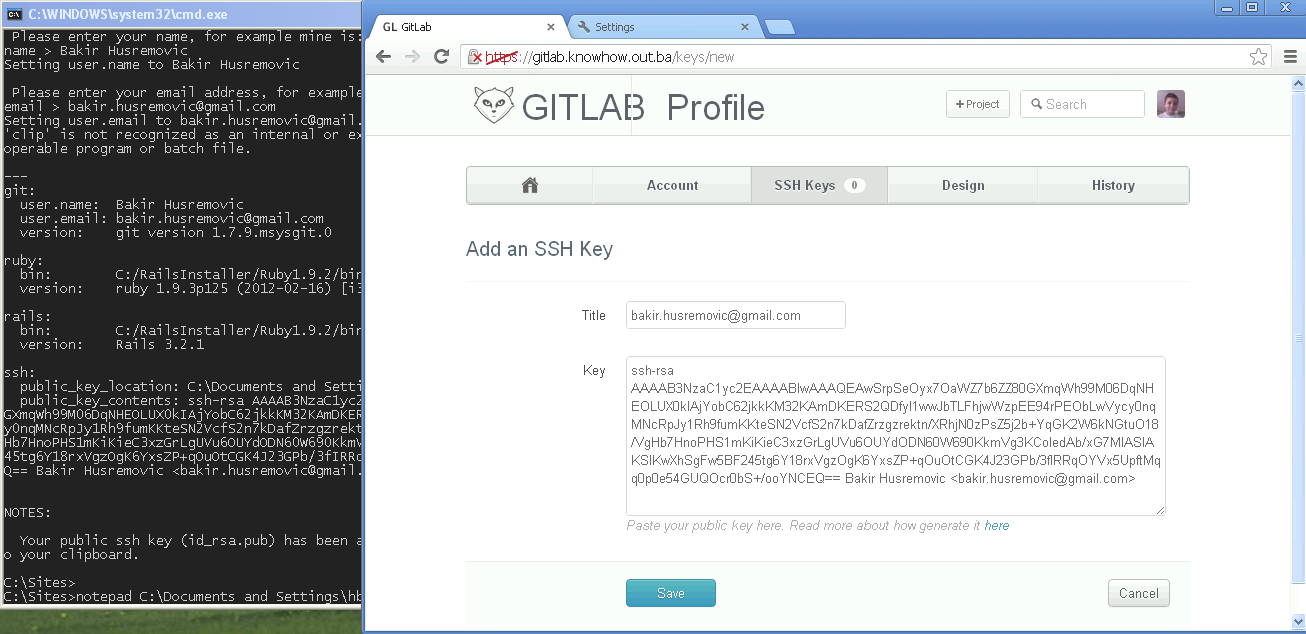
\includegraphics[width=15cm]{img/gitlab_ssh_profile.png}
\caption{Gitlab ssh profil}
\end{figure}

\chapter{Git workflow}

\section{Novi projekat}

Nakon podešenja ssh ključa, možemo kreirati naš prvi projekat ''helo\_ruby'':

\begin{figure}[H]
\centering
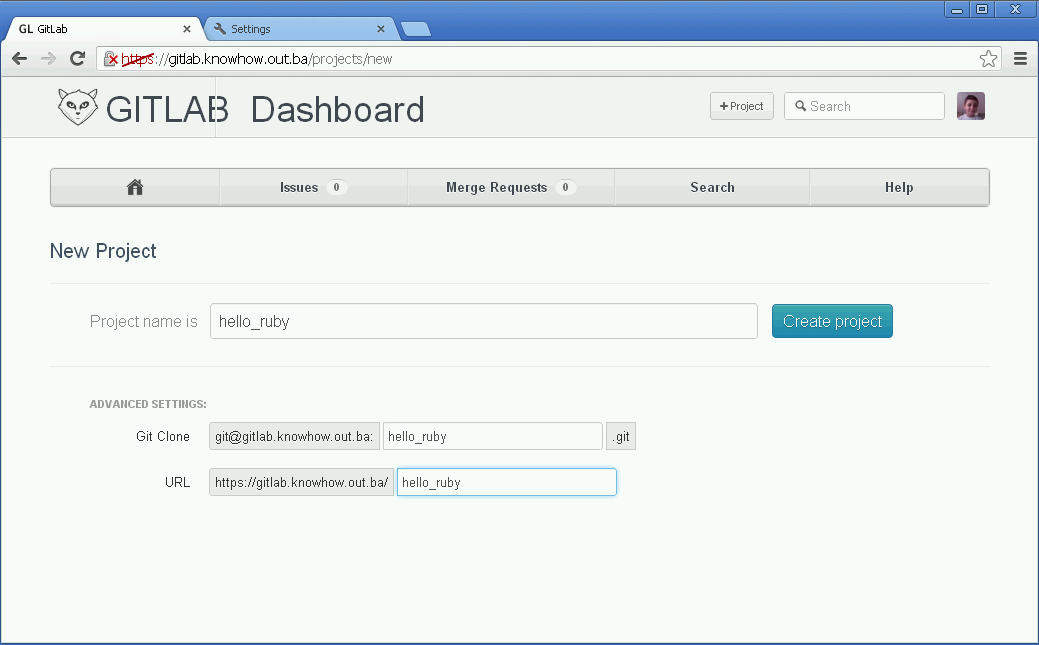
\includegraphics[width=15cm]{img/gitlab_new_project.png}
\caption{Gitlab: novi projekat}
\end{figure}

\begin{figure}[H]
\centering
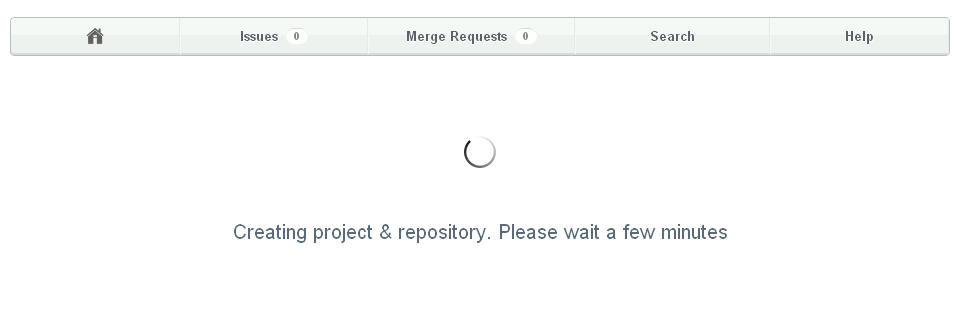
\includegraphics[width=15cm]{img/gitlab_new_project_2.png}
\caption{Gitlab: novi projekat - kreiranje git repozitorija}
\end{figure}

Nakon što je git repozitorij kreiran, dobijamo informacije o operacijama koje se obavljaju na remote klijentu za kreiranje i pristup git repozitoriju:

\begin{figure}[H]
\centering
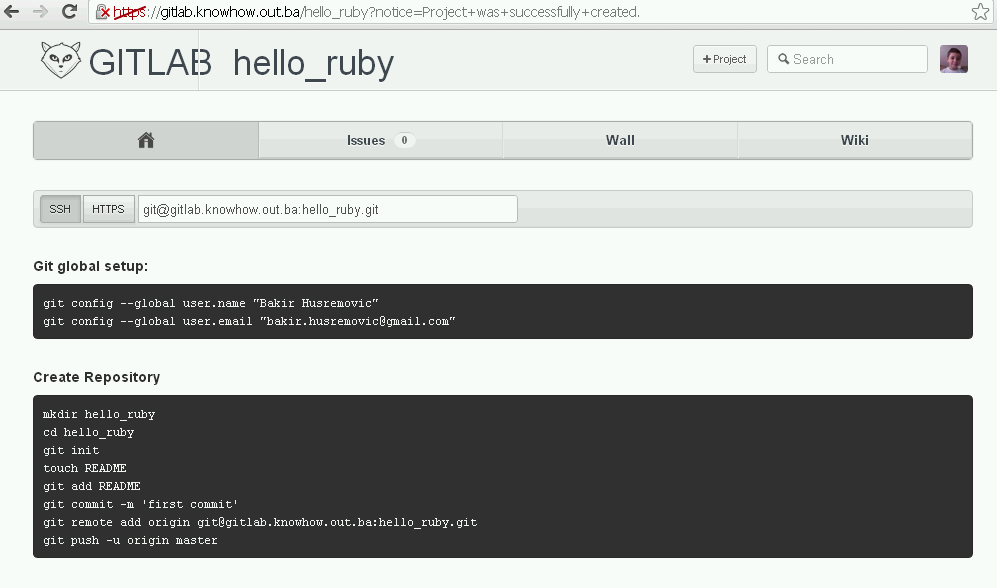
\includegraphics[width=15cm]{img/gitlab_new_project_3.png}
\caption{Gitlab: informacije o pristupu git prepozitiriju}
\end{figure}

\section{Development}

Na ''gitlab'' serveru je sve spremno za rad na našem prvom projektu. Napomenimo da u ovom trenutku na projektu radi samo jedan developer - Bakir. Kao kreator, on je ujedno i vlasnik projekta.

\subsection{Prvi ''commit''}

Slijedi rad na developerskoj radnoj stanici. Bakir će na svom "Windows" desktopu napraviti git repozitorij, te u njega smjestiti prvu verziju aplikacije.

\begin{figure}[H]
\centering
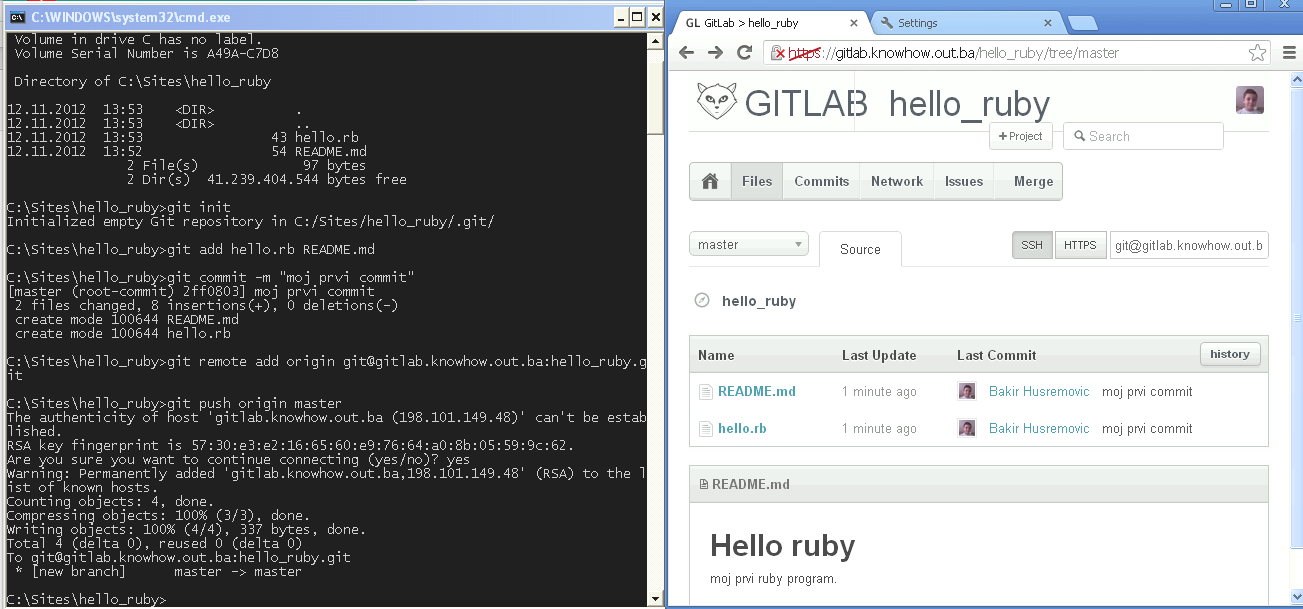
\includegraphics[width=15cm]{img/gitlab_first_commit.png}
\caption{Prve operacije na git repozitoriju: init, add, commit, push}
\end{figure}

Na konzoli su napravljeni prvi testovi hello.rb programa. Takođe, na gitlab web konzoli je nakon "push" operacije programski kod ''stigao'' i na server:

\begin{figure}[H]
\centering
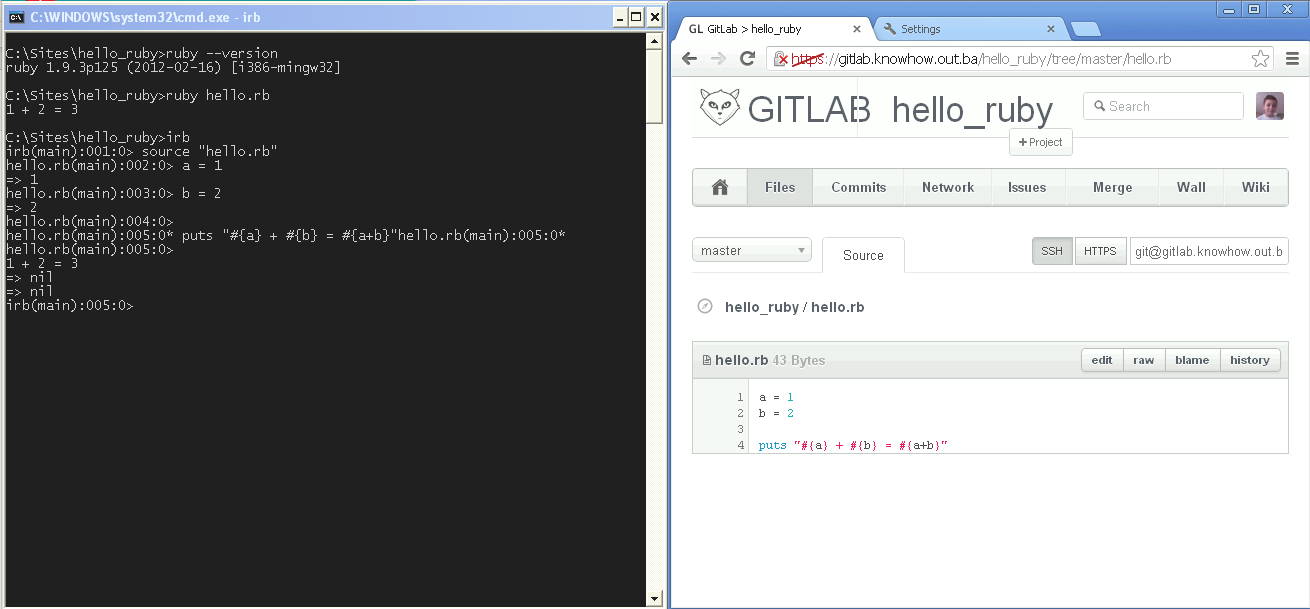
\includegraphics[width=15cm]{img/gitlab_first_commit_2.png}
\caption{Izvorni kod programa na gitlab serveru}
\end{figure}

\begin{figure}[H]
\centering
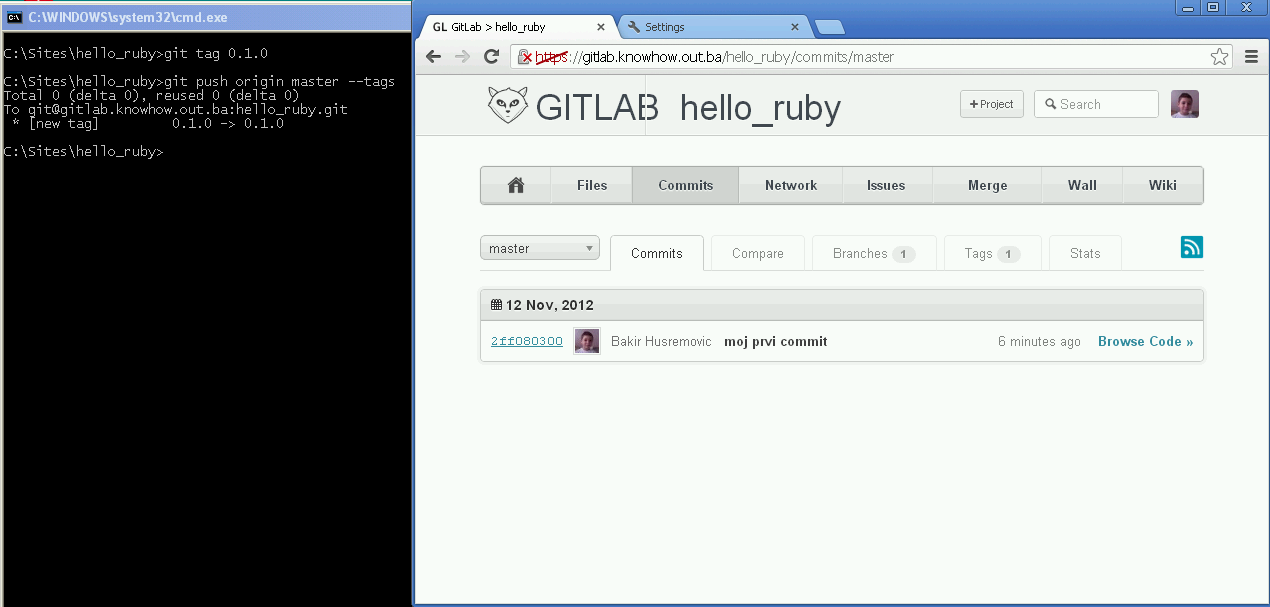
\includegraphics[width=15cm]{img/gitlab_tag_first_release.png}
\caption{''Označavamo'' prvu verziju našeg software-a: release 0.1.0}
\end{figure}

Napravimo pregled do sada izvršenih operacija:
\begin{enumerate}
  \item \texttt{git init} - kreiramo .git direktorij, lokalni git repozitorij
  \item \texttt{git remote add origin} - navodimo lokaciju našeg udaljenog - serverskog git repozitorija 
  \item \texttt{git add <ime fajla>} - dodajemo fajlove u lokalni repozitorij
  \item \texttt{git commit} - sve što unutar projekta dodali/promijenili smještamo u lokalni repozitorij
  \item \texttt{git tag} - ''tagiramo'' (označavamo) verziju 0.1.0
  \item \texttt{git push origin master} - šaljemo master\footnote{novokreirani git repozitorij uvijek ima ''master'' branch - to je podrazumjevani (eng. default) branch} ''branch'' na server 
\end{enumerate}

\subsection{Kreriranje novog ''branch''-a}

Nakon što je realizovao prvu verziju, Bakir kreće u izradu varijante aplikacije koja će moći preuzeti parametre sa komandne linije.

Pretpostavimo da se o zahtjevnom programskom zahvatu (rad tokom više radnih dana). Iz tog razloga ćemo otvoriti poseban branch ''parametri''.
Na taj način će tokom rada na ''parametar'' branch-u ''master'' branch ostati funkcionalan.


\setlength{\parindent 0cm}
Kreiramo novi branch:

C:/Sites/hello\_ruby> \texttt{git branch parametri}
\begin{lstlisting}
  origin/HEAD -> origin/master
  origin/master
  origin/parametri
\end{lstlisting}

Prebacujemo se na rad sa ''parametri'' branch-om.

C:/Sites/hello\_ruby> \texttt{git checkout parametri}
\begin{lstlisting}
Branch parametri set up to track remote branch parametri from origin.
Switched to a new branch 'parametri'
\end{lstlisting}

Pišemo novu verziju aplikacije, pa je testiramo.

Tokom pisanja nove verzije aplikacije, vršimo ''commit'' promjena u lokalni repozitorij:

\begin{figure}[H]
\centering
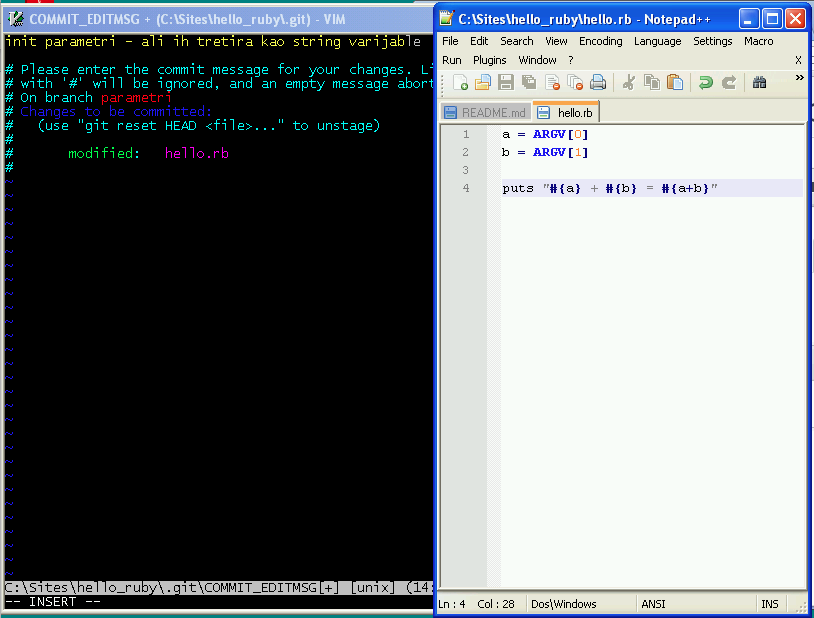
\includegraphics[width=15cm]{img/gitlab_new_branch_commit_with_vim}
\caption{git commit, unos ''commit'' poruke sa ''vim'' editorom}
\end{figure}

''Commit'' se vrši nakon svakog značajnijeg seta promjena na projektu.  Između dva ''commit''-a ne treba praviti velike pauze. Poželjno je da vrijeme između dva commit-a ne bude duže od par sahata. Treba izbjegavati velike ''commit''-e. Dugački commiti su teški za praćenje i otklanjanje grešaka.

\begin{figure}[H]
\centering
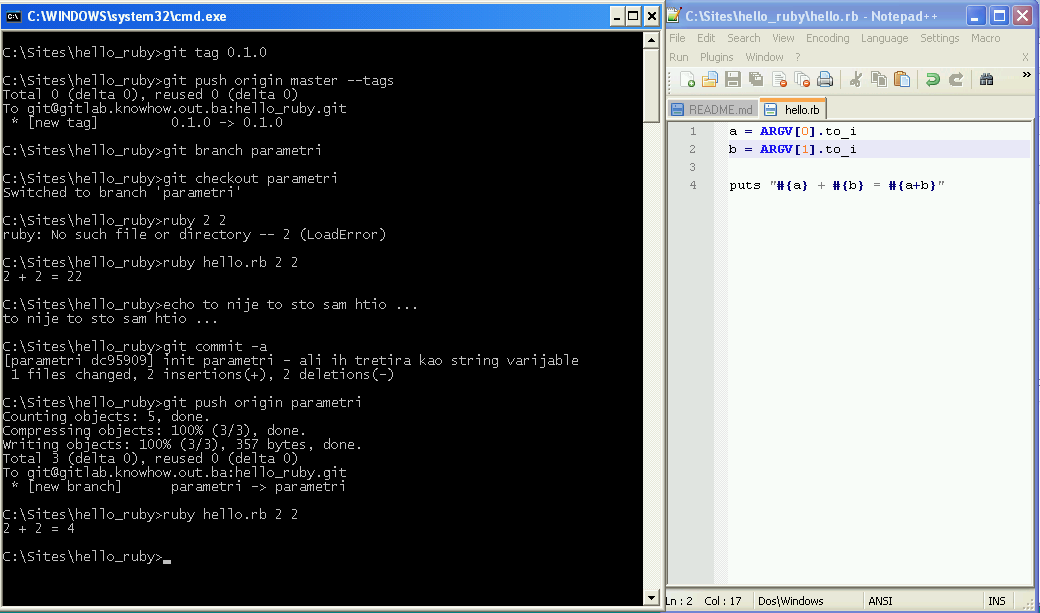
\includegraphics[width=15cm]{img/gitlab_new_branch_3.png}
\caption{Testiranje aplikativnog koda ''parametri'' branch-a}
\end{figure}

Kada smo završili sa pisanjem nove verzije aplikacije, vršimo ''push'' na server:

\begin{figure}[H]
\centering
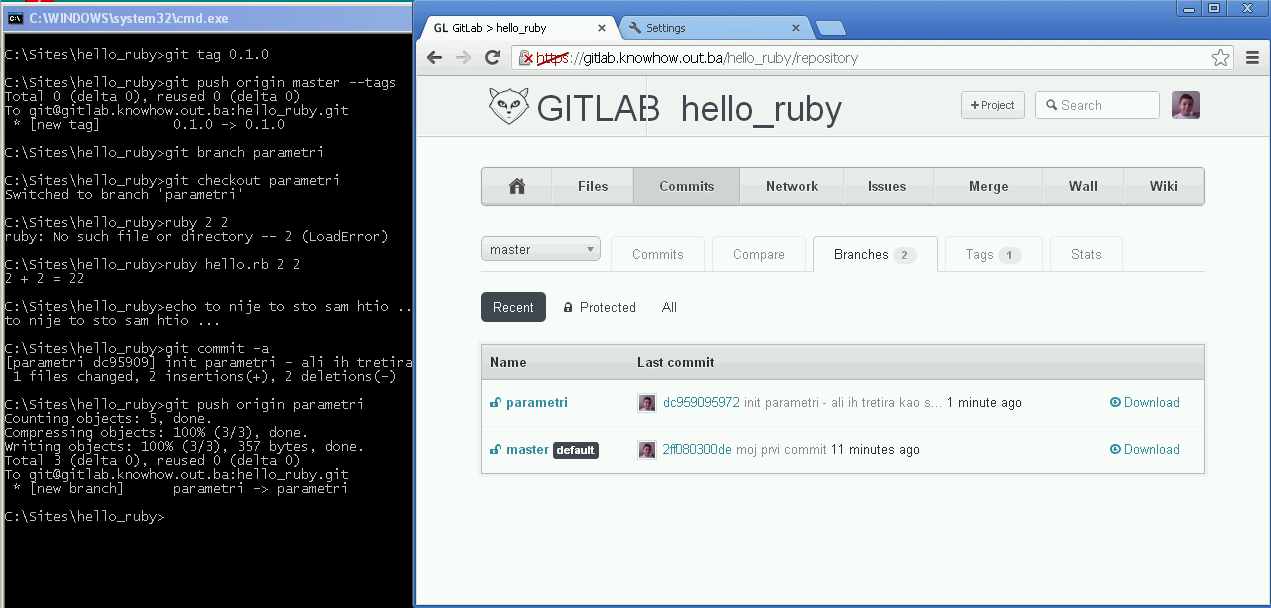
\includegraphics[width=15cm]{img/gitlab_new_branch.png}
\caption{Novi branch ''parametri'' na gitlab-u}
\end{figure}

Na web konzoli vidimo sve brach-ove i tag-ove našeg projekta:

\begin{figure}[H]
\centering
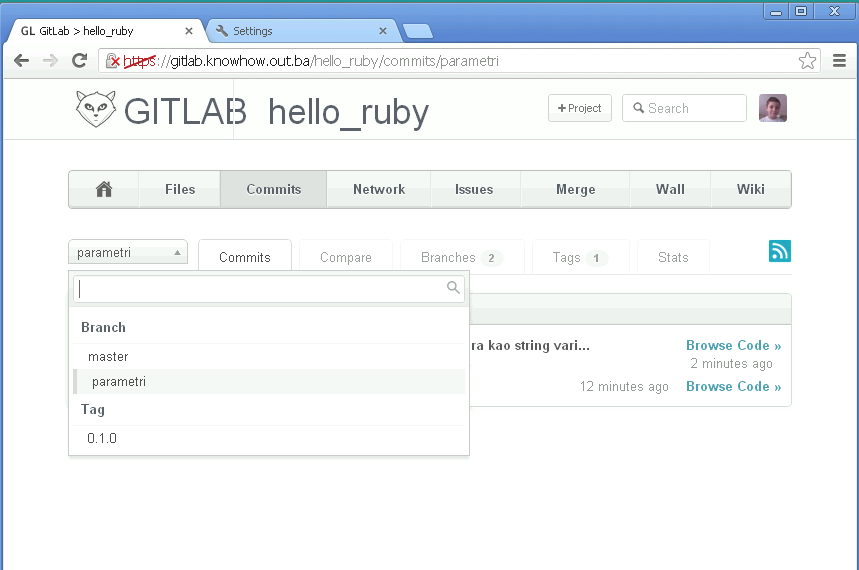
\includegraphics[width=15cm]{img/gitlab_new_branch_2.png}
\caption{Gitlab - pregled ''branch''-ova i ''tag''-ova}
\end{figure}

Kada se pozicioniramo na branch, vidimo sve ''commit''-e izvršene na tom branch-u:

\begin{figure}[H]
\centering
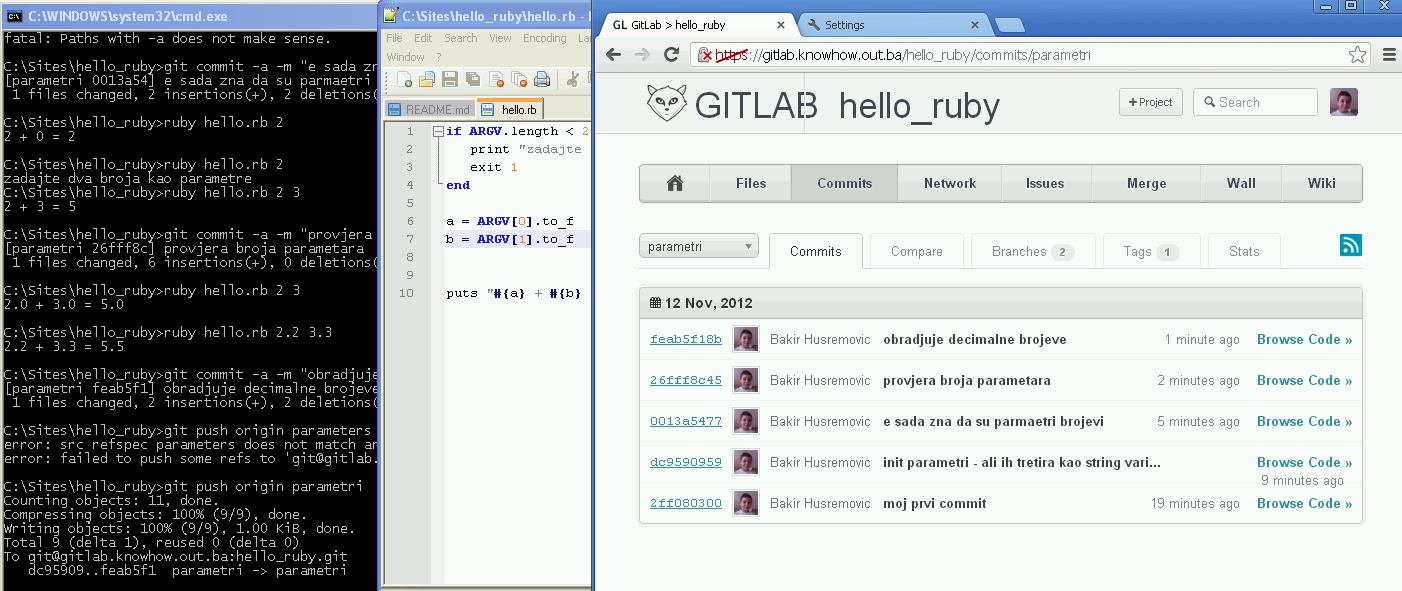
\includegraphics[width=16cm]{img/gitlab_new_branch_4_commits.png}
\caption{Gitlab commit-i na parametar branch-u}
\end{figure}

\subsection{''Merge'' promjena između dva ''branch''-a}

Nakon što su planirane operacije unutar ''parametar'' branch-a završene, promjene integrišemo u glavni - ''master'' branch.

To vršimo na sljedeći način:
\begin{enumerate}
  \item \texttt{git checkout master} - prebacujemo se na ''master'' brach
  \item \texttt{git merge parametri} - vršimo vršimo ''merge'' (spajajnje, integraciju) promjena iz ''parametri'' u  master branch
  \item \texttt{git tag 0.2.0} - označavamo verziju 0.2.0
  \item \texttt{git push master --tags} - pushiramo master branch, sa tagom na server
\end{enumerate}

Na gitlab serveru provjeravamo da li su promjene ''došle'' na server:

\begin{figure}[H]
\centering
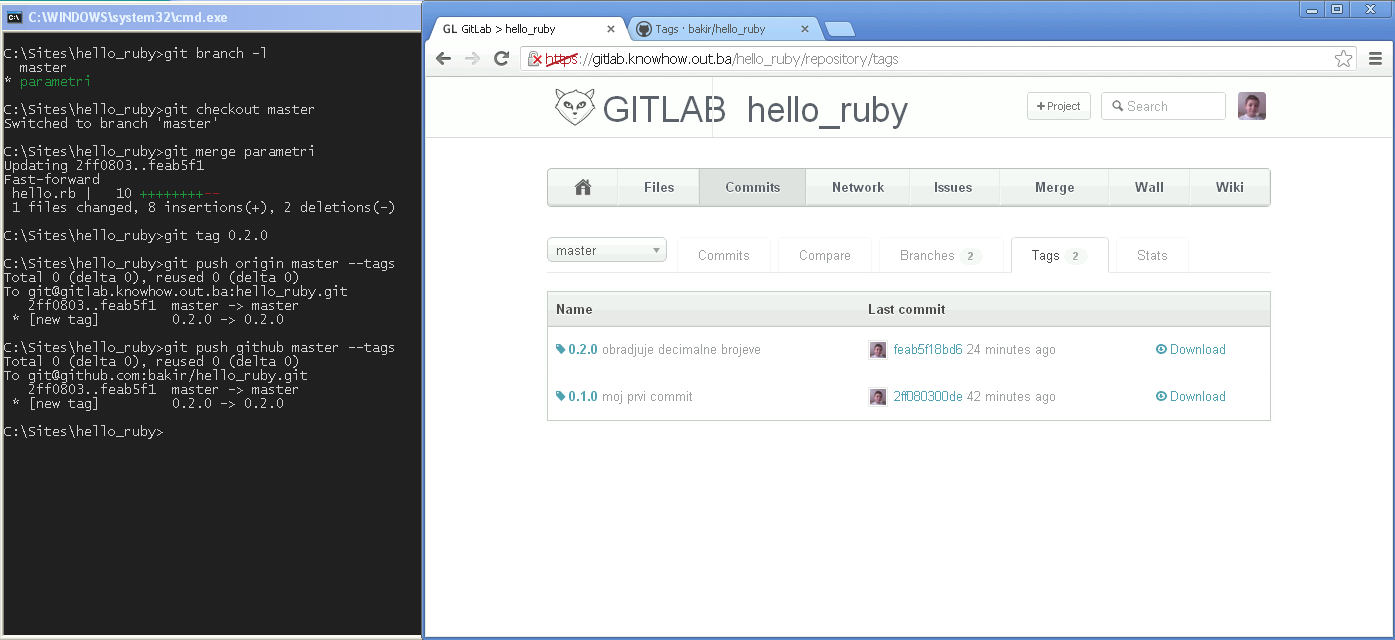
\includegraphics[width=16cm]{img/gitlab_tags.png}
\caption{Gitlab pregled tagova}
\end{figure}

Pregled svih operacija koje su do sada izvršene na projektu nalazi se na \href{https://gitlab.knowhow.out.ba/hello\_ruby}{\color{blue}{URL-u projekta}}:

\begin{figure}[H]
\centering
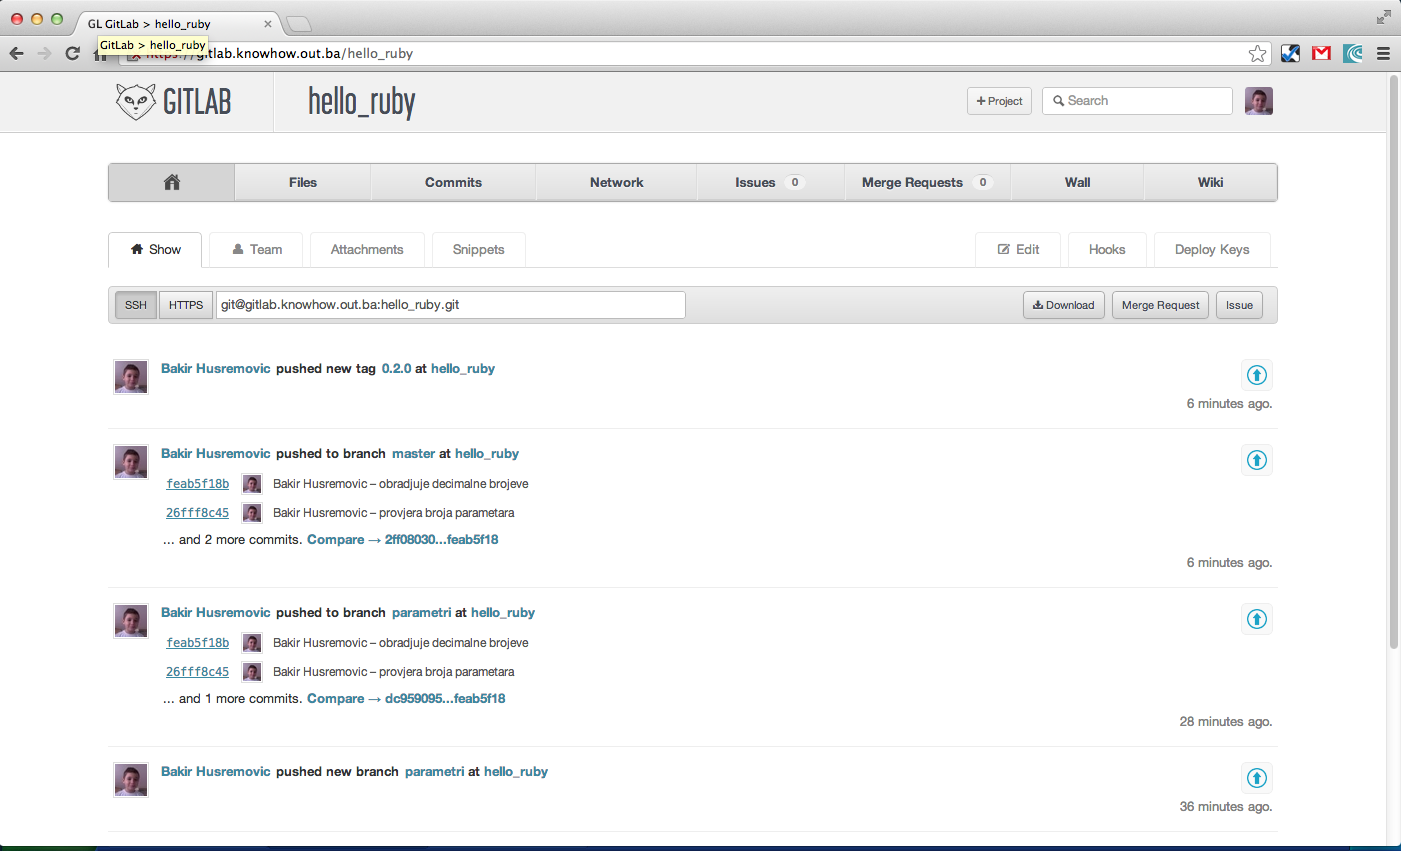
\includegraphics[width=15cm]{img/gitlab_project_show.png}
\caption{Glavne aktivnosti na projektu}
\end{figure}

\section{Public mirror ''hello\_ruby'' projekta na Github-u}

Glavni repozitorj projekta se nalazi na gitlab serveru. Međutim, ''gitlab'' ne omogućava anonimni pristup repozitorijima.

Ništa nas ne sprječava da na drugom git serveru kreiramo mirror našeg repozitorija.

To ćemo i učiniti. Otvorićemo account na github-u i na njemu kreirati hello\_ruby projekat.

\subsection{Github account}

Kreiranje novog korisničkog računa na github-u:

\begin{figure}[H]
\centering
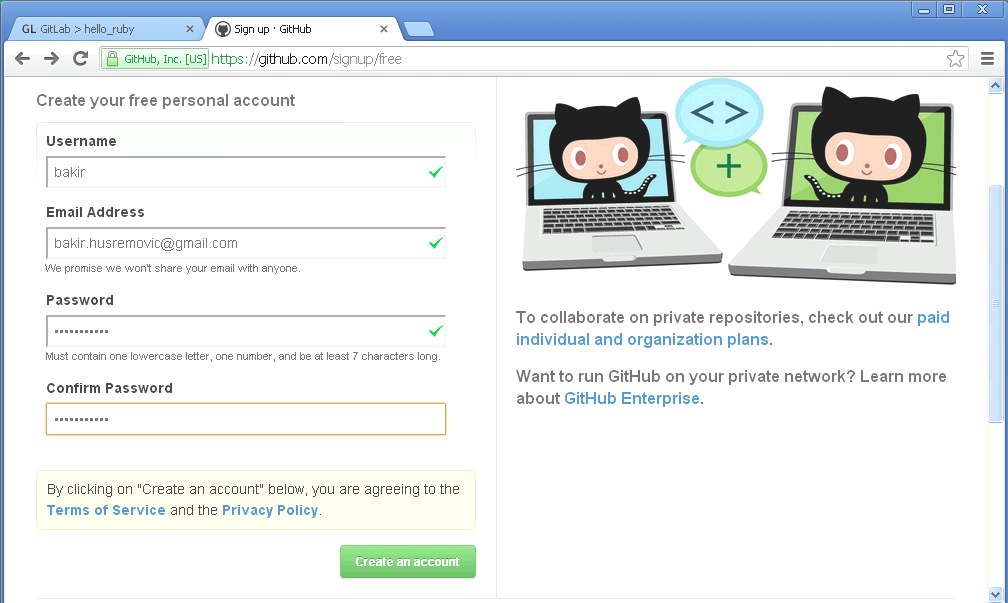
\includegraphics[width=15cm]{img/github_prijava.png}
\caption{Github prijava}
\end{figure}

\subsection{Github ssh postavke}

\begin{figure}[H]
\centering
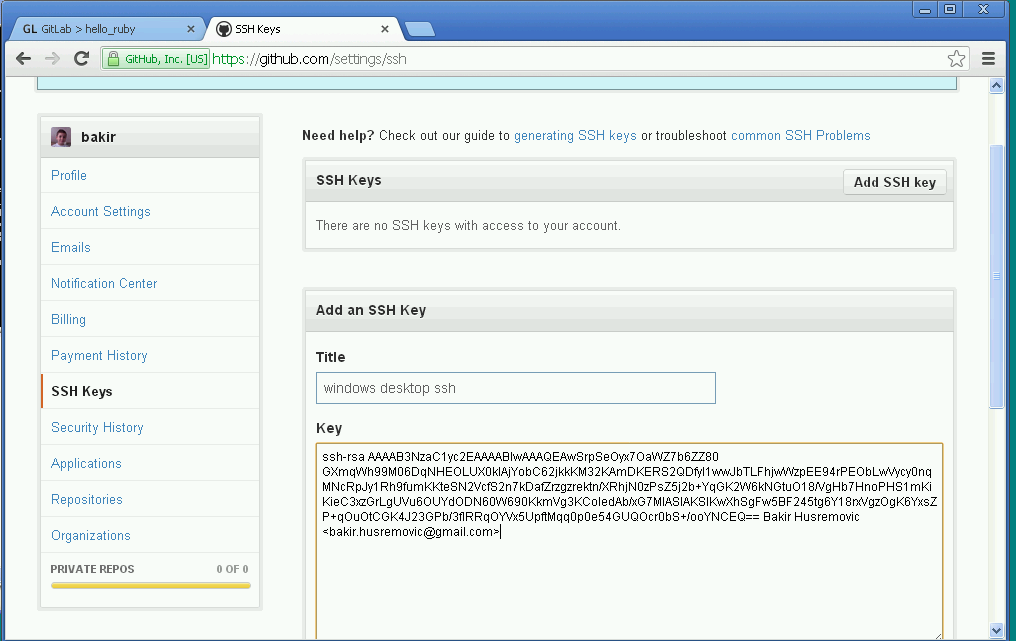
\includegraphics[width=15cm]{img/github_ssh_profile.png}
\caption{Github ssh profil}
\end{figure}

Ako razvoj obavlja na više radnih stanica, developer za svaku od njih dodaje poseban ssh ključ.

\begin{figure}[H]
\centering
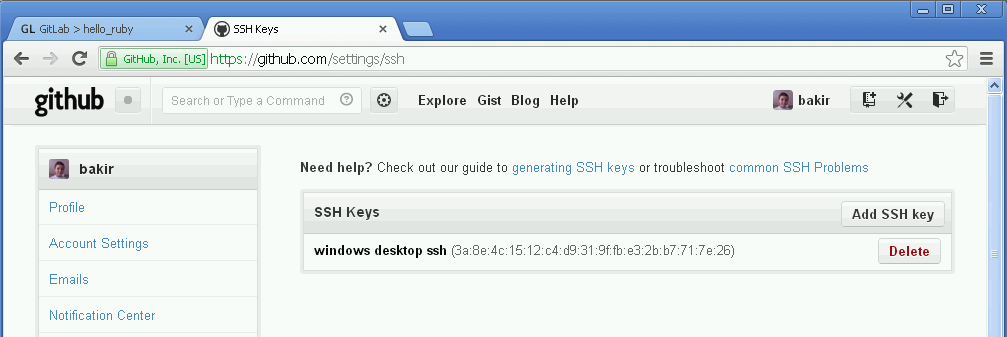
\includegraphics[width=15cm]{img/github_ssh_profile_2.png}
\caption{Github pregled aktivnih ssh ključeva}
\end{figure}

\subsection{Github kreiranje repozitorija}

\begin{figure}[H]
\centering
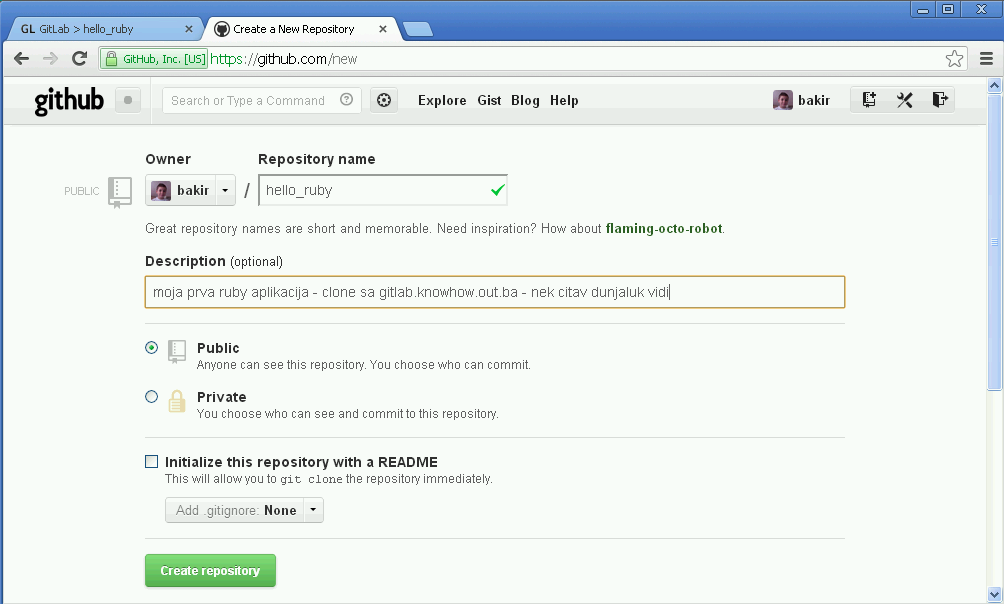
\includegraphics[width=15cm]{img/github_new_repos.png}
\caption{Github novi repozitorij}
\end{figure}

Nakon kreiranja servis nam prikazuje git operacije za uspostavljanje git repozitorija na radnoj stanici developera:

\begin{figure}[H]
\centering
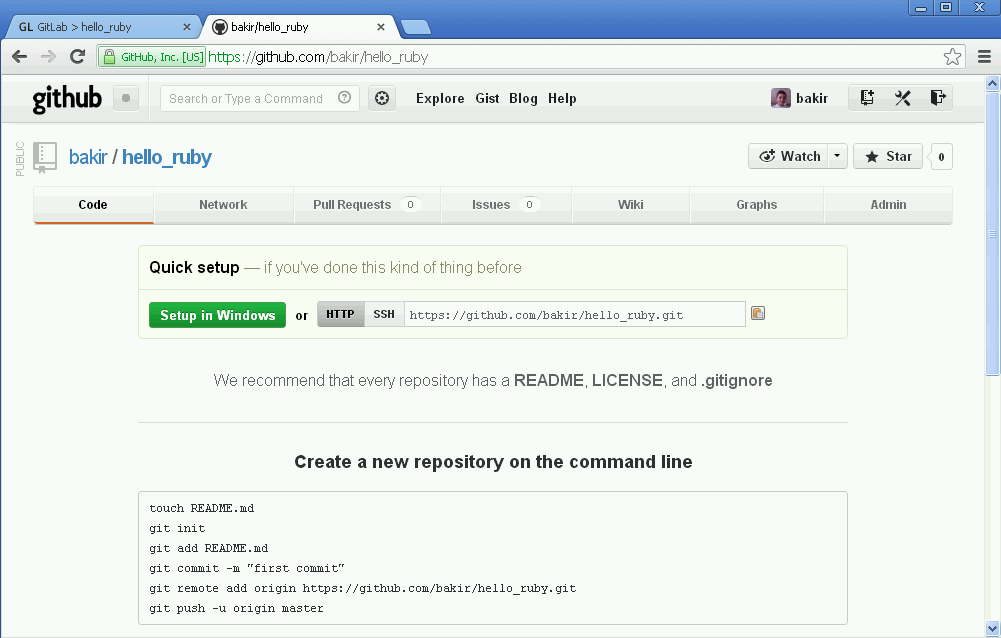
\includegraphics[width=15cm]{img/github_new_repos_2.png}
\caption{Github novi repozitorij - informacije o korištenju}
\end{figure}

\subsection{Kreiranje mirrora projekta na github-u}

S obzirom da mi već imamo remote ''origin'' koji ukazuje na gitlab server, radimo modifikaciju linija koje nam je predložio github:

\begin{enumerate}
  \item \texttt{git remote add github gitlab@github.com:bakir/hello\_ruby.git} - podesi github remote repozitorij
 \item \texttt{git push github master --tags} - pošalji master branch na github, zajedno sa tagovima
 \item \texttt{git push github parametri} - pošalji parametri branch na github
\end{enumerate}

\begin{figure}[H]
\centering
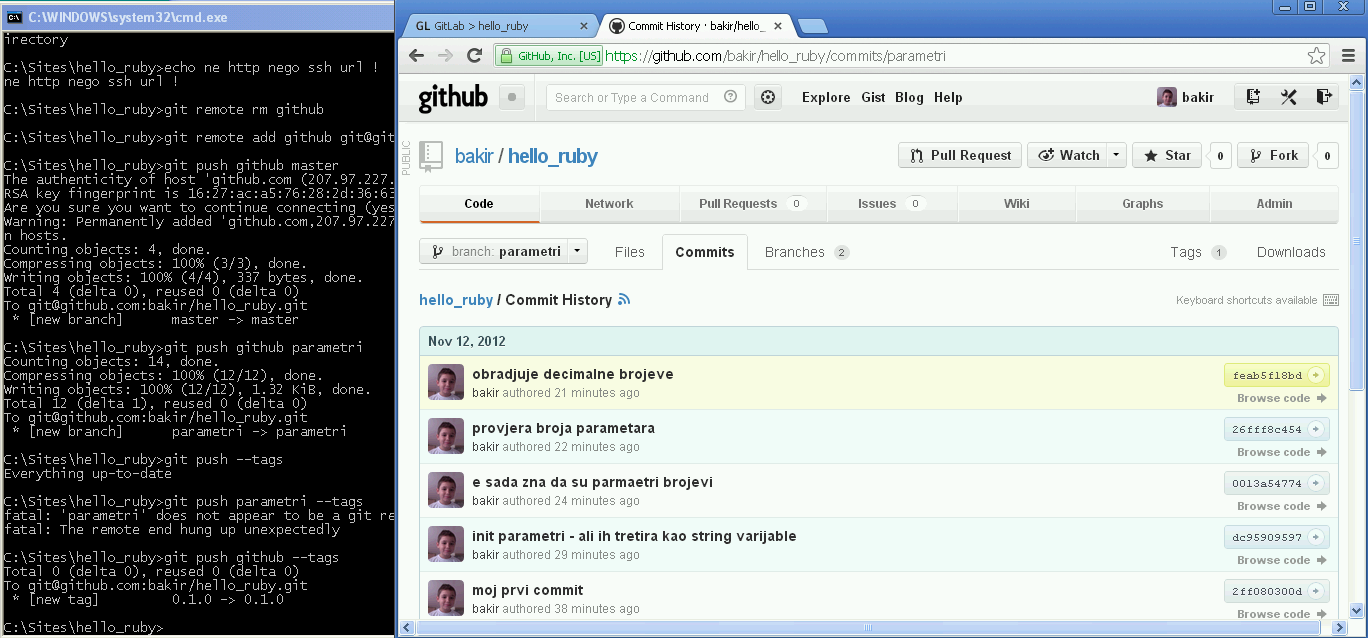
\includegraphics[width=15cm]{img/github_push_branches_and_tags.png}
\caption{Repozitorij na github-u nakon ''push'' operacija}
\end{figure}

Na kraju, imamo github mirror našeg projekta \url{https://github.com/bakir/hello\_ruby}

%\section{Nova verzija}

%Vrijeme je za novu verziju, zato vršimo tagiranje git repozitorija sa ''0.2.0'':

%\begin{figure}[H]
%\centering
%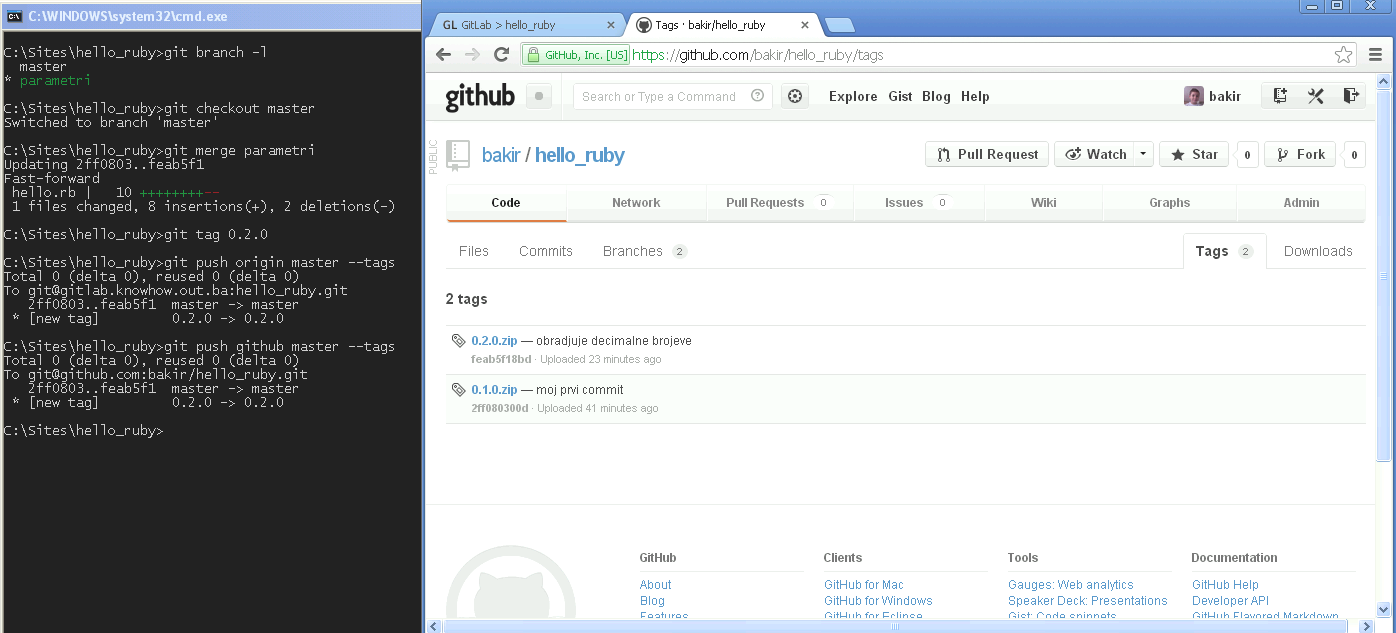
\includegraphics[width=16cm]{img/github_new_tag.png}
%\caption{Github - novi tag}
%\end{figure}


\section{Gitlab ''Diff'' funkcija}

Gitlab nam obezbjeđuje jednostavan pregled diff-ova (razlika) između različitih tačaka unutar git repozitorija.

Te tačke mogu biti stanje branch-a ili tag-a. Pogledajmo ''diff'' između verzija 0.1.0 i 0.2.0:

\begin{figure}[H]
\centering
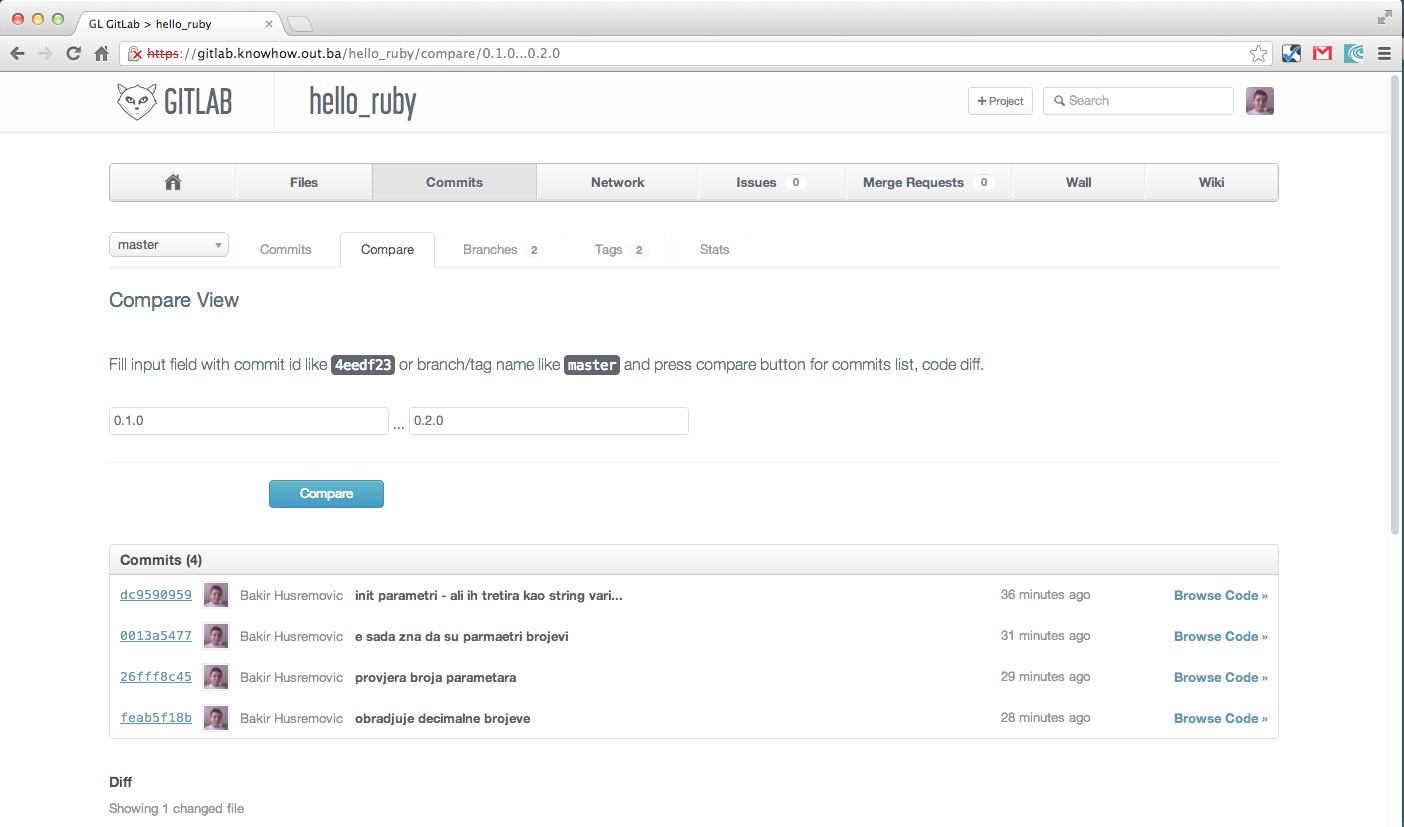
\includegraphics[width=15cm]{img/gitlab_compare.png}
\caption{Gitlab uporedi dvije verzije (dva tag-a)}
\end{figure}


\begin{figure}[H]
\centering
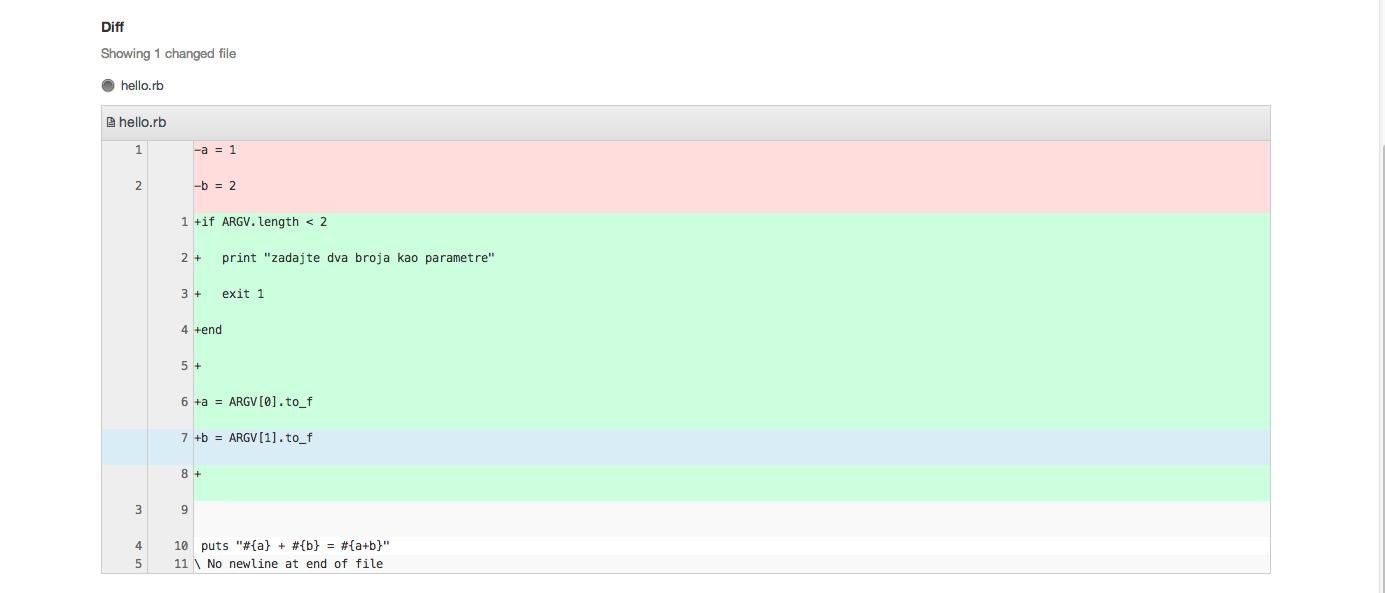
\includegraphics[width=15cm]{img/gitlab_compare_2.png}
\caption{Gitlab uporedi dvije verzije - diff}
\end{figure}


\section{Novi developer}

\subsection{Uključenje novog developera u projekat na gitlab-u}

Vlasnik projekta ''hello\_ruby'' Bakir uključuje novog developera Ernad u projekat:

\begin{figure}[H]
\centering
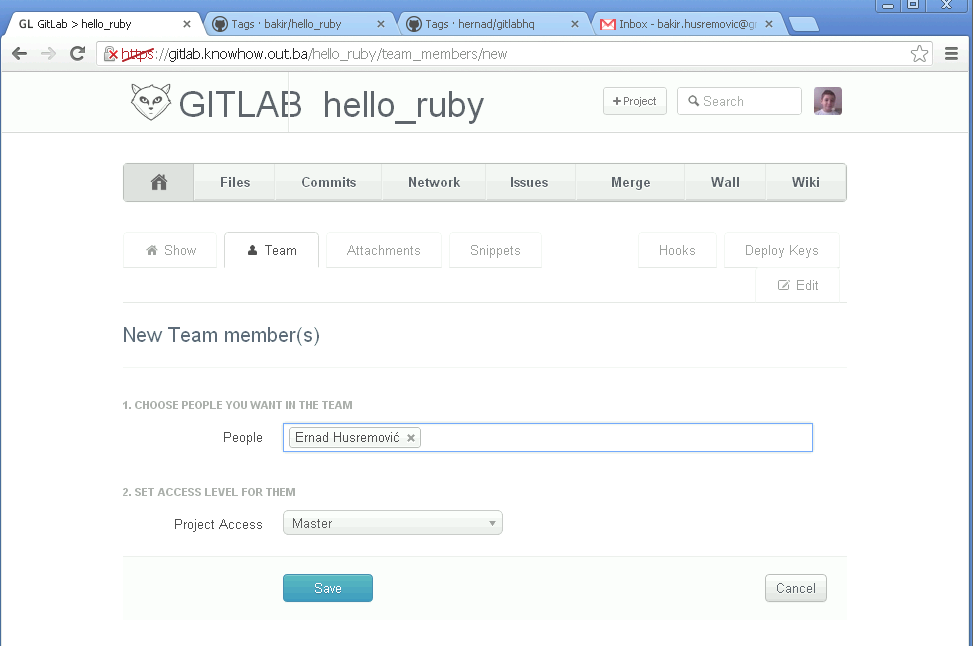
\includegraphics[width=15cm]{img/gitlab_add_new_member_to_project.png}
\caption{Gitlab: dodaj novog člana u projekat}
\end{figure}

Pri tome mu daje maksimalna prava (Master uloga).

\begin{figure}[H]
\centering
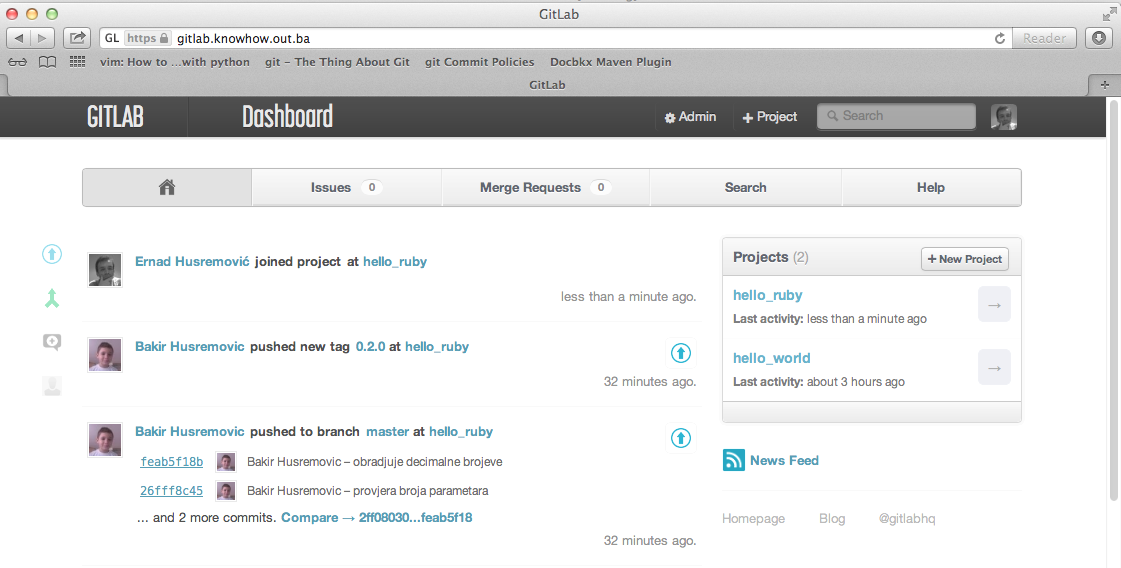
\includegraphics[width=15cm]{img/gitlab_add_new_member_to_project_2.png}
\caption{Gitlab dodaj novog člana u projekat 2}
\end{figure}

\subsection{Email notifikacija}

Developer primaju email notifikacije o svim bitnim događajima na projektu. Tako Ernad prima informaciju o uključenju u ''hello\_ruby'':

\begin{figure}[H]
\centering
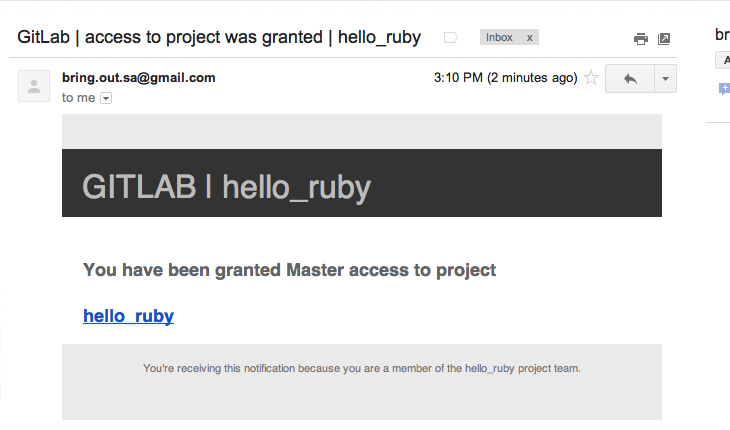
\includegraphics[width=15cm]{img/gitlab_email_notification.png}
\caption{Gitlab email notifikacija}
\end{figure}

\subsection{Kloniranje repozitorija}

\setlength{\parindent}{0cm}
Prvi korak novog developera je kloniranje repozitorija projekta na svoj desktop. 

Novi developer koristi Ubuntu linux desktop.

hernad@agile\_dev\_env\$ \newline
\texttt{git clone git@gitlab.knowhow.out.ba:hello\_ruby.git}
\begin{lstlisting}
Cloning into 'hello_ruby'...
remote: Counting objects: 16, done.
remote: Compressing objects: 100% (15/15), done.
remote: Total 16 (delta 1), reused 0 (delta 0)
Receiving objects: 100% (16/16), done.
Resolving deltas: 100% (1/1), done.
\end{lstlisting}

Pregled branch-ova na udaljenom repozitoriju:

hernad@hello\_ruby\$ \texttt{git branch -r}
\begin{lstlisting}
  origin/HEAD -> origin/master
  origin/master
  origin/parametri
\end{lstlisting}

\subsection{Novi developer, realizacija nove funkcije}

Ernad je senior developer. Uočava da njegov mladi kolega Bakir nije obradio bitne stavke kod obrade ulaznih parametara putem konzole.

Otvara novi branch ''babo'', da ne bi remetio stanje u glavnom branchu-u.

hernad@hello\_ruby\$ \texttt{git branch babo}

hernad@hello\_ruby\$ \texttt{git checkout babo}

\subsection{Git log}

Vrši niz promjena. Pregled tih promjena se može pogledati usa git log operacijom:

Pregled svog ''commit'' log-a:

hernad@hello\_ruby\$ \texttt{git log}
\begin{lstlisting}
commit 585688af924873852d72a0b9ccad16952c95fef0
Author: Ernad Husremovic <hernad@bring.out.ba>
Date:   Mon Nov 12 15:42:26 2012 +0100

    uputstvo

commit 71f0f17df4b4d0dcbca50034d638bc6bfae50424
Author: Ernad Husremovic <hernad@bring.out.ba>
Date:   Mon Nov 12 15:38:46 2012 +0100

    zaokruzenje pravi probleme
    
    ruby hello.rb
    treba zadati dva broja kao parametre aplikacije
    Unesite varijablu a: 1.1
    
    Unesite varijablu b: 2.2
    1.1 + 2.2 = 3.3000000000000003

commit 8e1c0bd154dd6a57d67266aee5f1f005c4aea603
Author: Ernad Husremovic <hernad@bring.out.ba>
Date:   Mon Nov 12 15:35:18 2012 +0100

    ako ne navedes parametre, procitaj ih sa konzole

commit feab5f18bd616ea7b4278024579e0a7aa728f448
Author: Bakir Husremovic <bakir.husremovic@gmail.com>
Date:   Mon Nov 12 14:15:45 2012 +0100

    obradjuje decimalne brojeve
\end{lstlisting}

Kada završi promjene, Ernad vrši ''push'' svog branch-a na server:

hernad@hello\_ruby\$ \texttt{git push origin babo}
\begin{lstlisting}
Counting objects: 12, done.
Delta compression using up to 8 threads.
Compressing objects: 100% (9/9), done.
Writing objects: 100% (9/9), 1.42 KiB, done.
Total 9 (delta 1), reused 0 (delta 0)
To git@gitlab.knowhow.out.ba:hello_ruby.git
 * [new branch]      babo -> babo
\end{lstlisting}

\section{Timski rad}
\subsection{Gitlab ''merge request''}

Ernad informiše bakira putem gitlab ''Merge request'' opcije od svom radu:

\begin{figure}[H]
\centering
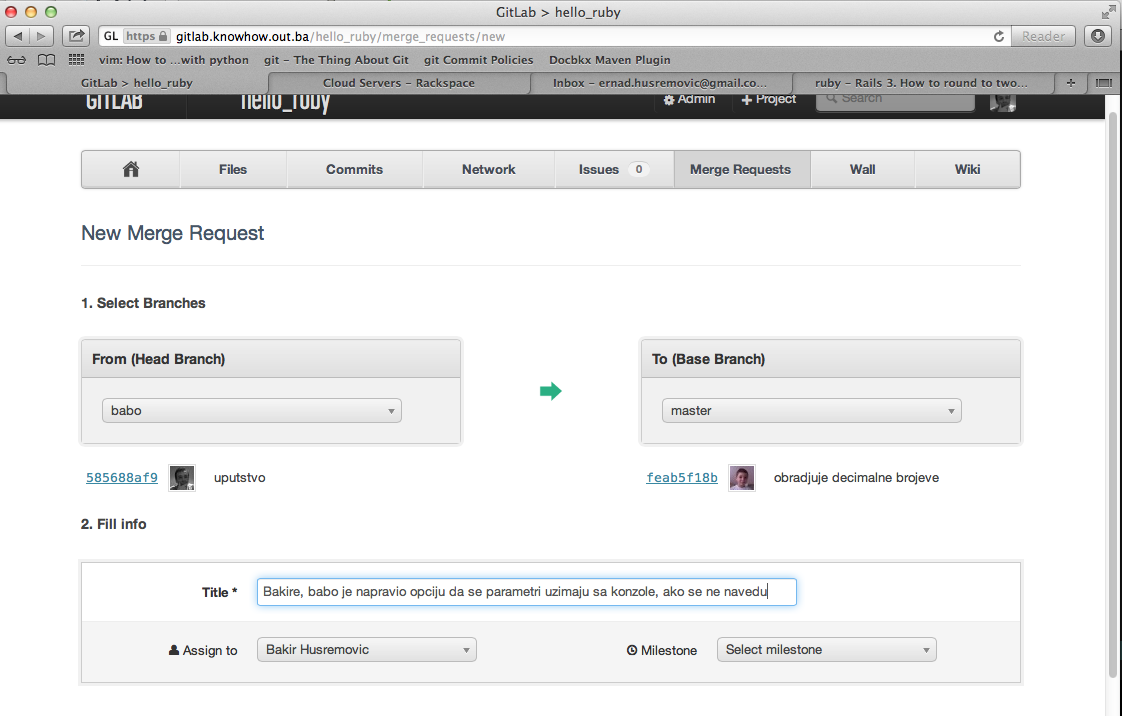
\includegraphics[width=14cm]{img/gitlab_merge_request.png}
\caption{Merge request}
\end{figure}

\begin{figure}[H]
\centering
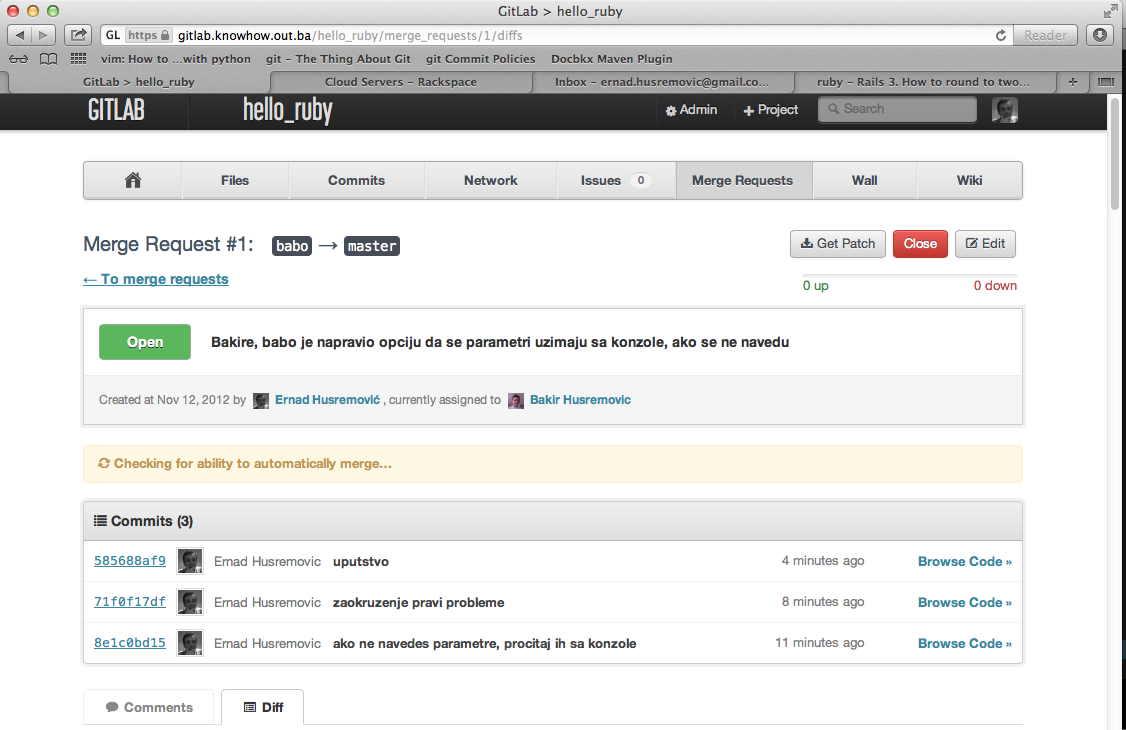
\includegraphics[width=14cm]{img/gitlab_merge_request_2.png}
\caption{Merge request}
\end{figure}

Bakir prima informaciju:

\begin{figure}[H]
\centering
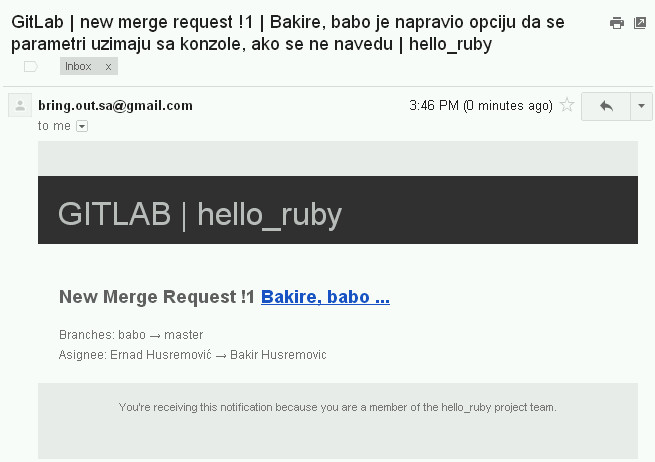
\includegraphics[width=12cm]{img/gitlab_merge_request_email_notification.png}
\caption{Bakir je o ''merge request''-u informisan putem email-a}
\end{figure}

Te odgovara pozitivno tako što vrši merge ''babo'' branch-a u ''master'' branch.
\begin{figure}[H]
\centering
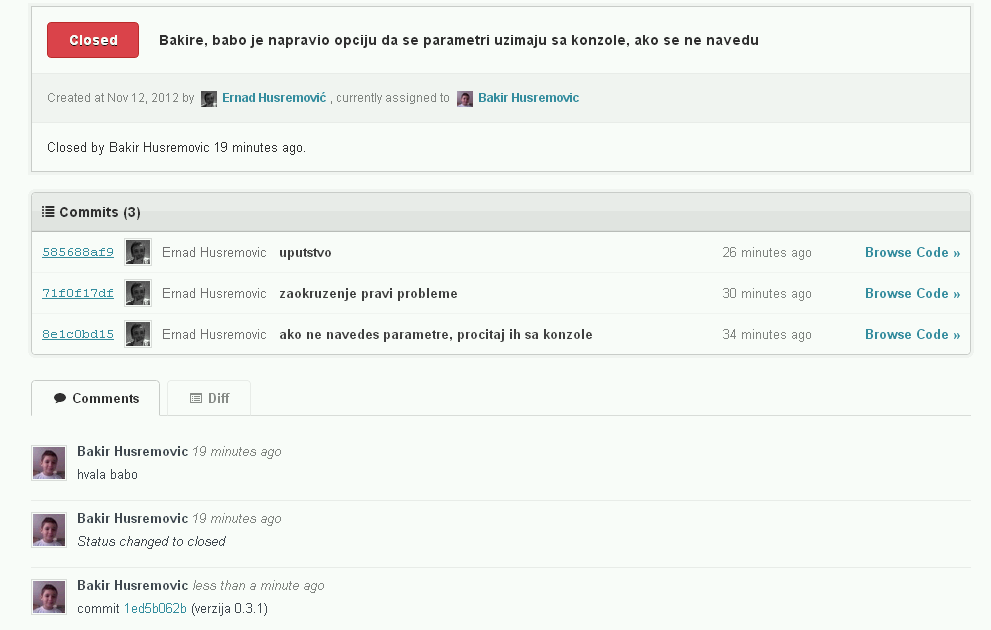
\includegraphics[width=15cm]{img/gitlab_merge_request_answer.png}
\caption{Merge request, Bakirov odgovor}
\end{figure}

\subsection{Git pull}

Git ''pull'' operacija uzima promjene sa servera. U slučaju novog branch-a, git klijent informiše o tome da se pojavio novi ''branch'', te da developer treba poduzeti odgovarajuće operacije da bi taj branch integrirao u svoj repozitorij:

C:/Sites/hello\_ruby> \texttt{git pull}
\begin{lstlisting}
remote: Counting objects: 12, done.
remote: Compressing objects: 100% (9/9), done.
remote: Total 9 (delta 1), reused 0 (delta 0)
Unpacking objects: 100% (9/9), done.
From gitlab.knowhow.out.ba:hello_ruby
 * [new branch]      babo       -> origin/babo
You asked me to pull without telling me which branch you
want to merge with, and 'branch.master.merge' in
your configuration file does not tell me, either. Please
specify which branch you want to use on the command line and
try again (e.g. 'git pull <repository> <refspec>').
See git-pull(1) for details.

If you often merge with the same branch, you may want to
use something like the following in your configuration file:
    [branch "master"]
    remote = <nickname>
    merge = <remote-ref>

    [remote "<nickname>"]
    url = <url>
    fetch = <refspec>

See git-config(1) for details.
\end{lstlisting}

Pregled svih udaljenih branchova:

C:/Sites/hello\_ruby> \texttt{git branch -r}
\begin{lstlisting}
  github/master
  github/parametri
  origin/babo
  origin/master
  origin/parametri
\end{lstlisting}

Bakir se operacijom ''checkout'' branch-a ''babo'' povezuje sa udaljenim branch-om istog imena:

C:/Sites/hello\_ruby> \texttt{git checkout babo}
\begin{lstlisting}
Branch babo set up to track remote branch babo from origin.
Switched to a new branch 'babo'
\end{lstlisting}

Njegov radni branch je sada ''babo'':

C:/Sites/hello\_ruby> \texttt{git branch -l}
\begin{lstlisting}
* babo
  master
  parametri
\end{lstlisting}

Međutim, on ne želi raditi na tom branchu, nego ga integrira u master branch operacijom git merge. Prvo se prebacuje na ''master'':

C:/Sites/hello\_ruby> \texttt{git checkout master}
\begin{lstlisting}
Switched to branch 'master'
\end{lstlisting}

pa onda vrši merge babo branch-a:

C:/Sites/hello\_ruby>git merge babo
\begin{lstlisting}
Updating feab5f1..585688a
Fast-forward
 README.md |   36 +++++++++++++++++++++++++++++++++++-
 hello.rb  |   38 ++++++++++++++++++++++++++++++++------
 2 files changed, 67 insertions(+), 7 deletions(-)
\end{lstlisting}

Bakir postavlja novu verziju aplikacije 0.3.0:

C:/Sites/hello\_ruby> \texttt{git tag 0.3.0}

Sve promjene koje je napravio (merge u master branch, novi tag 0.3.0) šalje na server:

C:/Sites/hello\_ruby> \texttt{git push github --tags}
\begin{lstlisting}
Counting objects: 21, done.
Compressing objects: 100% (18/18), done.
Writing objects: 100% (18/18), 2.37 KiB, done.
Total 18 (delta 4), reused 0 (delta 0)
To git@github.com:bakir/hello_ruby.git
 * [new tag]         0.3.0 -> 0.3.0
 * [new tag]         0.3.1 -> 0.3.1
\end{lstlisting}

\subsection{Brisanje privremenog ''branch''-a }

Nakon merdžiranja branch-a koji je bio privremene prirode, radi preglednosti vršimo njegovo brisanje.

Brišemo branch na lokalnom repozitoriju:

C:/Sites/hello\_ruby> \texttt{git branch babo -d}
\begin{lstlisting}
Deleted branch babo (was 585688a).
\end{lstlisting}

Pogledajmo pregled remote branchova-a:

C:/Sites/hello\_ruby> \texttt{git branch -r}
\begin{lstlisting}
  github/master
  github/parametri
  origin/babo
  origin/master
  origin/parametri
\end{lstlisting}

Brišemo i remote branch babo:

C:/Sites/hello\_ruby> \texttt{git branch -rd origin/babo}
\begin{lstlisting}
Deleted remote branch origin/babo (was 585688a).
\end{lstlisting}

Šaljemo promjene o brisanju na server. Naglašavamo operaciju ''delete'':

C:/Sites/hello\_ruby> \texttt{git push origin --delete babo}
\begin{lstlisting}
To git@gitlab.knowhow.out.ba:hello_ruby.git
 - [deleted]         babo
\end{lstlisting}

\section{''Collective code ownership''}

\begin{quotation}
  \emph{We are all responsible for high-quality code.}
\end{quotation}

''Collective code ownership''\citep[str. ]{agileart} je agilni princip po kome svako odgovoran za visoki kvalitet koda.
Ako se tokom čitanja uputstva uoče nedostaci, ako je programski kod nepregledan, pristupa se popravci.
Pri tome se ne gleda ko je originalni pisac uputstva ili koda. Kod je u vlasništvu tima.

Ernad je nakon Bakirovih intervencija na uputstvu uočio da postoji još par stavki koje bi trebalo ispraviti.

Za ovu intervenciju nema nikakvog razloga praviti novi branch - ispravke će se vršiti direktno u ''master''-u.

Ernad vrši update master-a na svom desktopu:

hernad@hello\ruby\$ \texttt{git checkout master}
\begin{lstlisting}
Switched to branch 'master'
Your branch is behind 'origin/master' by 6 commits, and can be fast-forwarded.
\end{lstlisting}

Ernad preuzima (pull-uje) Bakir-ove promjene sa servera:

hernad@hello\ruby\$ \texttt{git pull}
\begin{lstlisting}
Updating feab5f1..1ed5b06
Fast-forward
 README.md |   34 +++++++++++++++++++++++++++++++++-
 hello.rb  |   38 ++++++++++++++++++++++++++++++++------
 2 files changed, 65 insertions(+), 7 deletions(-)
\end{lstlisting}

Vršimo ispravku uputstva u našem editoru:
hernad@hello\ruby\$ \texttt{vi README.md}

Commit promjena:

hernad@hello\ruby\$ \texttt{git commit -a -m ''uputstvo update''}
\begin{lstlisting}
[master 74fb346] uputstvo update
 1 file changed, 1 insertion(+), 1 deletion(-)
\end{lstlisting}

Označava novu verziju 0.3.2:

hernad@hello\ruby\$ \texttt{git tag 0.3.2}

hernad@hello\ruby\$ \texttt{git push origin master --tags}
\begin{lstlisting}
Counting objects: 5, done.
Delta compression using up to 8 threads.
Compressing objects: 100% (3/3), done.
Writing objects: 100% (3/3), 333 bytes, done.
Total 3 (delta 1), reused 0 (delta 0)
To git@gitlab.knowhow.out.ba:hello_ruby.git
   1ed5b06..74fb346  master -> master
 * [new tag]         0.3.2 -> 0.3.2
\end{lstlisting}

Treba uočiti da je ovaj proces brz i jednostavan. Ne traži nikakve posebne dogovore između developera.
Jednostavno, svako ko uoči potrebu da napravi sitnu korekciju - to i čini.

\chapter{Git unutar IDE-a}

Git ima podršku za sve poznate IDE-alate:

\begin{itemize}
  \item Microsoft visual studio ''GIT Source Control Provider'' - \url{http://gitscc.codeplex.com}
  \item Jetbrains Idea - \url{http://www.jetbrains.com/idea/webhelp/using-git-integration.html}
  \item Netbeans - \url{http://netbeans.org/kb/docs/ide/git.html}
  \item Eclipse - \url{http://www.eclipse.org/egit}

\subsection{Eclipse IDE}

Instalacijom \href{http://www.vogella.com/articles/EGit/article.html}{\color{blue}{EGit plugin-a}} možemo unutar našeg IDE-a vršiti operacije nad git repozitorijom.

Untar našeg projekta podešavamo, git repozitorij (s obzirom da on već postoji):
\begin{figure}[H]
\centering
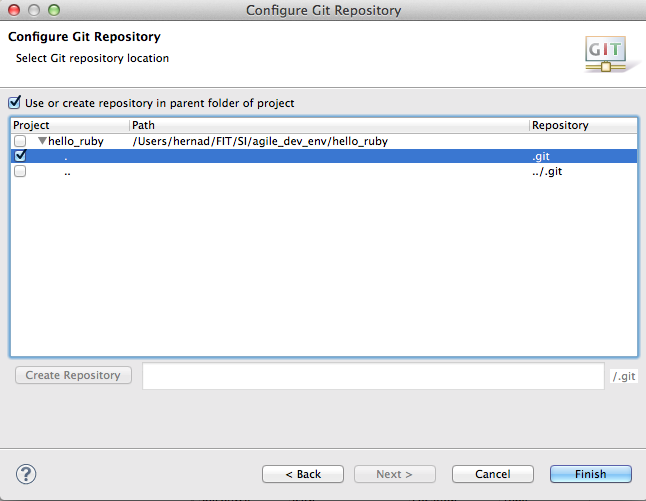
\includegraphics[width=10cm]{img/eclipse_git_01.png}
\caption{Eclipse IDE git - setup postojećeg repozitorija u IDE-u}
\end{figure}

Nakon toga su nam dostupne SCM operacije nad repozitorijom:
\begin{figure}[H]
\centering
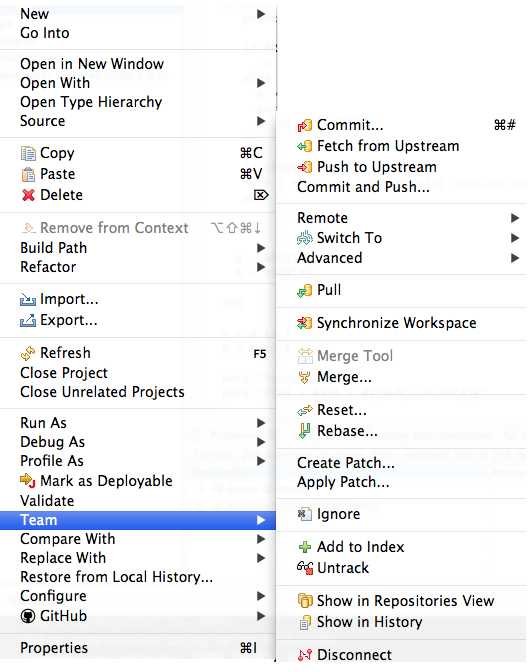
\includegraphics[width=8cm]{img/eclipse_git_02.png}
\caption{Eclipse IDE GIT - Project team support}
\end{figure}

Nakon izvršenih promjena unutar IDE-a, pokrećemo commit unutar IDE-a:
\begin{figure}[H]
\centering
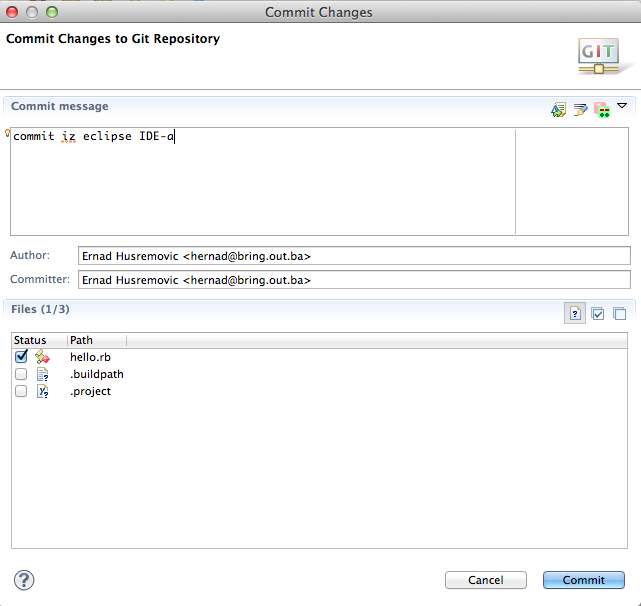
\includegraphics[width=10cm]{img/eclipse_git_03.png}
\caption{Eclipse IDE commit dijalog}
\end{figure}

Push na remote repozitorij:

\begin{figure}[H]
\centering
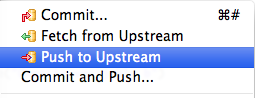
\includegraphics[width=4.5cm]{img/eclipse_git_04.png}
\caption{Eclipse push dijalog}
\end{figure}

\begin{figure}[H]
\centering
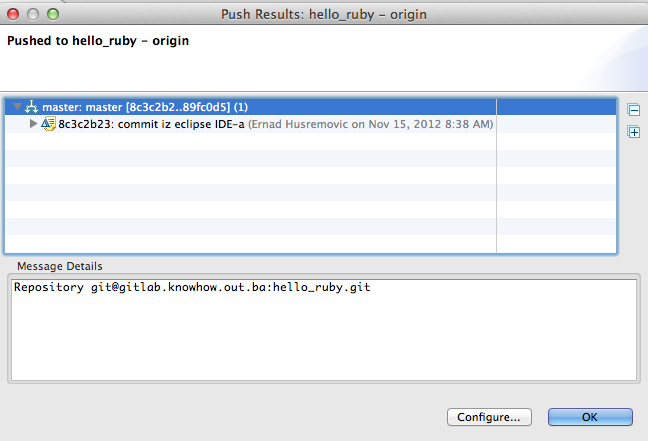
\includegraphics[width=10cm]{img/eclipse_git_05.png}
\caption{Eclipse IDE, informacija o izvršenoj push operaciji}
\end{figure}

\begin{figure}[H]
\centering
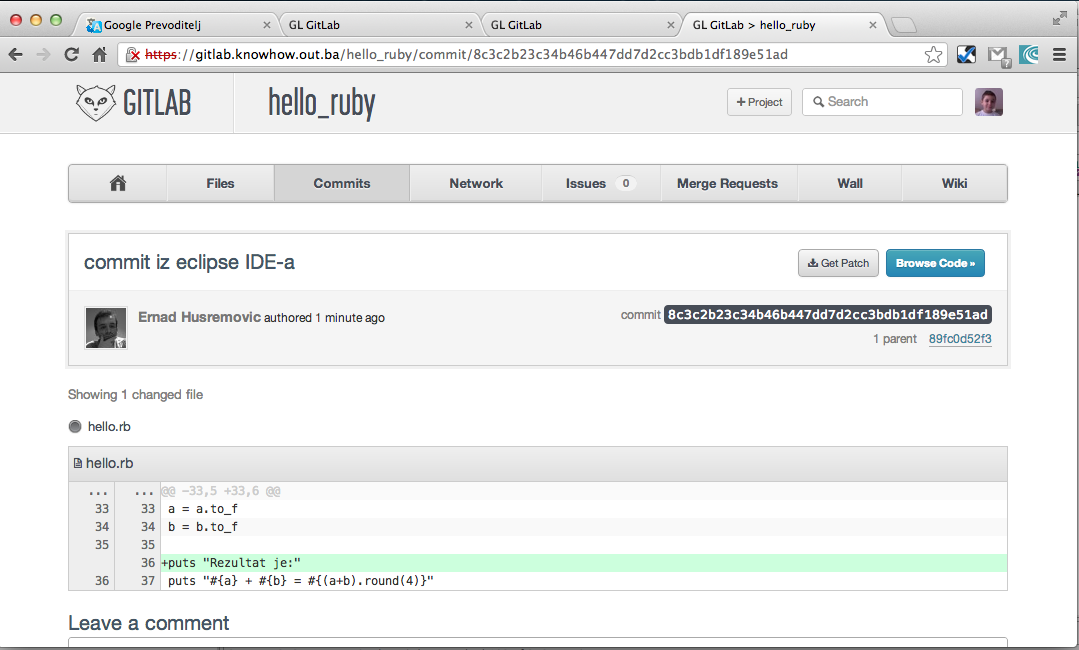
\includegraphics[width=15cm]{img/eclipse_git_06.png}
\caption{Naša promjena nalazi se na gitlab serveru}
\end{figure}


\chapter{Zaključak}

Git nam omogućava da se jedan od ključnih prinicipa agilnog sofware developmenta, \emph{''Collective code ownership''}, na najbolji način realizira u praksi.

Git omogućava developeru da sve svoje ideje sa minimalnim ''overhead''-om pohrani u centralni repozitorij (branching, merging).

Web servisi kao što su ''Github'' i ''Gitlab'' omogućavaju jednostavnu i efikasnu komunikaciju tima. Centralna tačka komunikacije je izvorni kod\footnote{Ovdje se misli na izvorni kod u širem smislu. Misli se na sve digitalne artifakte projekta. Dokumentacija je sastavni dio izvornog koda}.
Kako je izvorni kod projekta ujedno i glavni proizvod programskog tima, prirodno je da to bude centralno mjesto komunikacije.

Pored mogućnosti da se direktno ispravlja programski kod, svaki član tima ima mogućnost komentara pojedinih ''commit''-a.

Ta opcija omogućava iskusnijim članovima tima (senior developer, ''product manager'', ''agile couch''\citep{agileart}) da mlađim kolegama brzo i jednostavno daju upute za korekcije i nadogradnju njihovog koda.


%\begin{center}
%\emph{\large{Freedom to create, distribute, and use open source software (OSS).}}
%\end{center}


% -------------------------------------------------
\bibliography{literatura}
\bibliographystyle{fit}

% -------------------------------------------------
\appendix

\chapter{Riječnik pojmova}

\begin{itemize}
    \item \texttt{tag} - tag je oznaka unutar git repozitorija koja najčešće pokazuje na određenu verziju (release) ili podverziju - iteraciju (iteration)

    \item \texttt{branch} - branch označava poseban ogranak projekat u odnosu na glavni tok razvoja. Primjera radi, ako želimo uvesti neke eksperimentalne funkcije, otvaramo poseban "experimental" branch unutar koga implementiramo naše eksperimentalne funkcije. Te promjene se ne vide na glavnom - ''master'' branch-u.
    \item \texttt{merge request} - Proces merdžiranja (eng. merge - spojiti) je proces u kome se vrši spajanje promjena iz različiti branch-ova ili različitih repozotorija. Vezano za primjer branch-a (vidi: branch), ako su se promjene u ''experimental'' branch-u pokazale dobrim, ''merge'' operacijom ih prebacujemo - integriramo u ''master'' branch. Nakon uspješnog merdžiranja ''experimental'' branch možemo obrisati.
    \item \texttt{repository} - baza u promjena. Lokalni repozitorij se nalazi u .git repozitoriju našeg projekta na lokalnom disku. 'Remote' repozitorij se uobičajeno nalazi na udaljenom serveru kome pristupamo putsem ssh ili http protokola.
    \item \texttt{diff} - Skraćenica od ''difference''. Koristi se za poređenje dva različita stanja repozitorija. Tačka poređenja mogu biti ''tag'', ''branch'' ili jednostavno određeni ''commit''.
\end{itemize}

\chapter{Napomene}

Materijal je prepun anglizama, što odstupa od uobičajenih akademskih standarda pisanja. Međutim, s obzirom na ciljni auditorij, mišljenja smo da bi pokušaj prevođenja na maternji jezik izazvao više konfuzije nego što bi pomogao u razumjevanju sadržaja.

Uzmimo za primjer \href{http://translate.google.com/#en/hr/commit}{\color{blue}{''commit''}} operaciju.
''Commit'' operacijom se promjene šalju - predaju u lokalni repozitorij.
Stoga je prevod ''predaj'' vjerovatno najpogodniji. Međutim, kada bi takav prevod prevod izvršili na na sljedećem ekranu:

\begin{figure}[H]
\centering
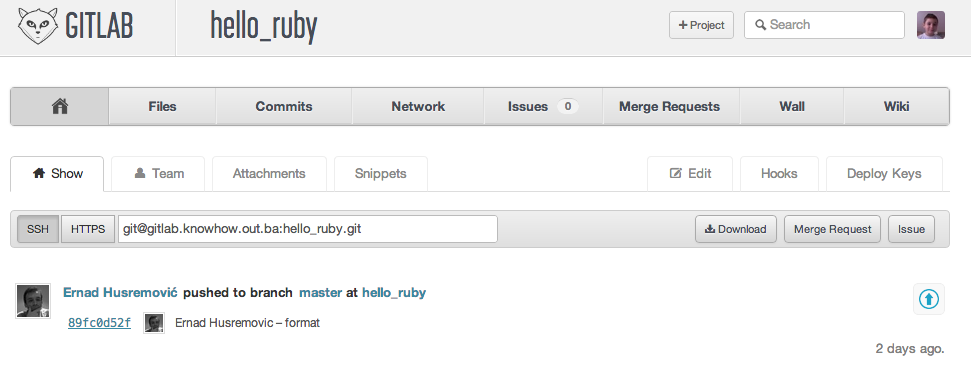
\includegraphics[width=14cm]{img/cik_prevedi.png}
\caption{Prevod na bosanski - nemoguća misija}
\end{figure}

dobili bi više-manje nerazumljiv sadržaj. Pored toga, developerski alati nisu lokalizirani. Stoga bi developer tokom korištenja alata (npr. git klijenta) stalno vršio dodatnu operaciju prevoda (predaj -> commit). To je razlog zbog koga se termini ''commit'', ''push'', ''merge'', ''branch'' u materijalu koriste isključivo u izvornoj formi - na engleskom jeziku, ili pominju kao anglizmi (merdžiranje, puširanje i sl.). Jednostavno, korištena je terminologija kojom uobičajeno služe developeri. Može se reći da je ovakvo izražavanje u skladu sa principom agilnog software developmenta ''Ubiquitous Language''\citep[str. 125]{agileart} 


developera. jezik developera, koliko god on '

\chapter{Software toolset}
\begin{enumerate}
  \item Mac OS X 10.8.2
  \item mvim, vim tekst editor ver 7.3
  \item MacTex (TeX Live 2012)
\end{enumerate}

\chapter{Software repozitoriji}

\begin{itemize}
  \item Agilni developerski environment  \url{https://github.com/hernad/agile\_dev\_env}
  \item Gitlab instalacija
  \begin{itemize}
       \item Gitlab repozitorij \url{https://github.com/hernad/gitlabhq}
       \item Vagrant/Chef recepies \url{https://github.com/hernad/vagrant\_gitlab}}
       \item Instalacija servera na rackspace cloud server \url{https://github.com/hernad/ubuntu\_bootstrap\_chef}
  \end{itemize}
  \item Git repozitorij koji je obrađen u materijalu \url{https://github.com/bakir/hello\_ruby}
  \item Gitlab primjer repozitorij\footnote{potreban login pristup gitlab serveru} \url{https://gitlab.knowhow.out.ba/hello\_ruby}
\end{itemize}

\end{document}
